% =============================================================================
% LLM-Augmented Network Intrusion Detection Using the Model Context Protocol
% Thesis Draft — Deep Analysis, Notes, and Draft Sections
% University of Queensland — Dual Degree (EE Mechatronics + CS)
% =============================================================================
\documentclass[12pt, a4paper, oneside]{report}

% ── Packages ─────────────────────────────────────────────────────────────────
\usepackage[utf8]{inputenc}
\usepackage[T1]{fontenc}
\usepackage{lmodern}
\usepackage[margin=2.5cm]{geometry}
\usepackage{graphicx}
\usepackage{booktabs}
% \usepackage{multirow}  % removed — replaced with manual row spans
\usepackage{array}
\usepackage{amsmath, amssymb}
\usepackage{xcolor}
\usepackage{csquotes}
\usepackage[style=numeric, backend=biber, sorting=none]{biblatex}
\addbibresource{references.bib}
\usepackage{hyperref}
% \usepackage{cleveref}  % requires extra install; use \ref{} instead
\usepackage{enumitem}
\usepackage{float}
\usepackage{caption}
\usepackage{listings}
\usepackage{algorithm}
\usepackage{algpseudocode}
\usepackage{pgfplots}
\pgfplotsset{compat=1.18}
\usepackage{tikz}
\usetikzlibrary{positioning, arrows.meta, shapes.geometric, calc}

% ── Colours ──────────────────────────────────────────────────────────────────
\definecolor{UQpurple}{HTML}{51247A}
\definecolor{accent}{HTML}{2E86AB}
\definecolor{codegreen}{HTML}{2E7D32}
\definecolor{codegray}{HTML}{6C757D}
\definecolor{codeblue}{HTML}{1565C0}

\hypersetup{
  colorlinks=true,
  linkcolor=UQpurple,
  citecolor=accent,
  urlcolor=accent
}

% ── Listing style ────────────────────────────────────────────────────────────
\lstset{
  basicstyle=\ttfamily\small,
  keywordstyle=\color{codeblue}\bfseries,
  commentstyle=\color{codegray}\itshape,
  stringstyle=\color{codegreen},
  breaklines=true,
  frame=single,
  rulecolor=\color{codegray!40},
  xleftmargin=1em,
  framexleftmargin=0.5em,
  numbers=left,
  numberstyle=\tiny\color{codegray},
  showstringspaces=false
}

% ── Custom commands ──────────────────────────────────────────────────────────
\newcommand{\tmark}{\textsuperscript{$\dagger$}}
\newcommand{\metric}[1]{\textbf{#1}}
\newcommand{\todo}[1]{\textcolor{red}{\textbf{[TODO: #1]}}}
\newcommand{\note}[1]{\textcolor{accent}{\textit{[Note: #1]}}}

% ── Title ────────────────────────────────────────────────────────────────────
\title{%
  \vspace{-2cm}
  {\Large University of Queensland}\\[0.5em]
  {\large School of Electrical Engineering and Computer Science}\\[2em]
  {\LARGE\bfseries LLM-Augmented Network Intrusion Detection\\
  Using the Model Context Protocol}\\[1.5em]
  {\large Thesis Draft --- Deep Analysis \& Working Sections}\\[1em]
}
\author{%
  Kunwar Singh\\
  Dual Degree: Electrical Engineering (Mechatronics) / Computer Science\\[0.5em]
  \textit{Supervisor:} \todo{TBD}
}
\date{February 2026}

% =============================================================================
\begin{document}
\maketitle
\tableofcontents
\newpage


% #############################################################################
% PART I — DEEP ANALYSIS OF EXPERIMENTAL RESULTS
% #############################################################################
\part{Deep Analysis of Experimental Results}
\label{part:analysis}


% =============================================================================
\chapter{Phase 1: MCP-Augmented Single-Agent Evaluation}
\label{ch:phase1-analysis}
% =============================================================================

\section{Experiment Configuration}

The baseline evaluation used an autonomous ReAct-loop agent (Claude 3.5 Sonnet,
\texttt{claude-sonnet-4-20250514}) connected to 13 MCP tools via STDIO transport.
The agent processed each flow independently---no memory persisted between flows.

\begin{table}[H]
\centering
\caption{Phase 1 experiment configuration}
\label{tab:phase1-config}
\begin{tabular}{@{}ll@{}}
\toprule
\textbf{Parameter} & \textbf{Value} \\
\midrule
Model             & Claude 3.5 Sonnet (\texttt{claude-sonnet-4-20250514}) \\
MCP tools         & 13 (5 external intel, 3 MITRE, 5 NetFlow analyzer) \\
Test batch        & 58 flows, 4 stratified tiers \\
Dataset           & CICIDS2018 NetFlow v3 (development split) \\
Transport         & STDIO (MCP server spawned as subprocess) \\
Memory            & None (each flow analysed in isolation) \\
\bottomrule
\end{tabular}
\end{table}

\subsection{Tiered Test Batch Design}

The 58-flow batch was stratified into four tiers to isolate the contribution of
different tool categories:

\begin{enumerate}[label=\textbf{Tier \arabic*:}, leftmargin=3.5em]
  \item \textbf{External-tool-testable} (9 flows) --- Flows with public IPs
        (18.x.x.x, 13.x.x.x, 52.x.x.x) that \emph{should} return data from
        AbuseIPDB, OTX, and geolocation APIs. Included FTP brute force and SSH
        brute force attacks.
  \item \textbf{Feature-rich attacks} (22 flows) --- High-volume attacks
        (DDoS-HOIC, LOIC-UDP/HTTP, DoS-GoldenEye, Hulk, SlowHTTPTest,
        Slowloris) where flow-level statistics alone carry strong signal.
        IN\_BYTES 232$\times$ and IN\_PKTS 599$\times$ attack/benign ratio.
  \item \textbf{Temporal-context attacks} (12 flows) --- Low-and-slow attacks
        (Brute Force XSS, SQL Injection, Infiltration) whose individual flows
        resemble benign traffic. Detection requires cross-flow temporal
        correlation.
  \item \textbf{Benign baseline} (15 flows) --- Legitimate DNS, DHCP, HTTPS
        traffic. Tests the false-positive rate.
\end{enumerate}


% ─────────────────────────────────────────────────────────────────────────────
\section{Overall Results}
\label{sec:phase1-results}

\begin{table}[H]
\centering
\caption{Phase 1 binary classification performance (Attack vs.\ Benign)}
\label{tab:phase1-overall}
\begin{tabular}{@{}lrr@{}}
\toprule
\textbf{Metric} & \textbf{Value} & \textbf{Count} \\
\midrule
Accuracy   & 72.4\% & 42 / 58 \\
Precision  & 75.5\% & 40 / 53 \\
Recall     & 93.0\% & 40 / 43 \\
F1 Score   & 83.3\% & --- \\
\midrule
True Positives  & --- & 40 \\
True Negatives  & --- & 2 \\
False Positives & --- & 13 \\
False Negatives & --- & 3 \\
\midrule
Benign Accuracy & 13.3\% & 2 / 15 \\
\bottomrule
\end{tabular}
\end{table}

\subsection{Per-Tier Performance}

\begin{table}[H]
\centering
\caption{Phase 1 per-tier metrics}
\label{tab:phase1-tiers}
\begin{tabular}{@{}lccccccc@{}}
\toprule
\textbf{Tier} & \textbf{Flows} & \textbf{Acc.} & \textbf{Prec.} & \textbf{Rec.}
  & \textbf{F1} & \textbf{Tools/Flow} & \textbf{Cost/Flow} \\
\midrule
1. External-testable  &  9 & 100.0\% & 100.0\% & 100.0\% & 100.0\% & 4.4 & \$0.070 \\
2. Feature-rich       & 22 & 100.0\% & 100.0\% & 100.0\% & 100.0\% & 4.1 & \$0.068 \\
3. Temporal-context   & 12 &  75.0\% & 100.0\% &  75.0\% &  85.7\% & 4.0 & \$0.066 \\
4. Benign baseline    & 15 &  13.3\% &   0.0\% &   0.0\% &   0.0\% & 4.0 & \$0.071 \\
\bottomrule
\end{tabular}
\end{table}


% ─────────────────────────────────────────────────────────────────────────────
\section{Deep Interpretation of Phase 1 Numbers}
\label{sec:phase1-interpretation}

\subsection{Why Recall is High (93.0\%) but Accuracy is Low (72.4\%)}

The agent exhibits a \emph{suspicious-by-default} bias: it classified 53 out of 58
flows as attack/suspicious, yielding 40 true positives but also 13 false positives
(all benign flows misclassified). The high recall reflects the agent's tendency to
flag anything uncertain as suspicious rather than benign.

The confusion matrix is asymmetric: only 2 of 15 benign flows were correctly
identified (\metric{13.3\% benign accuracy}). This is the single most important
failure mode---the agent cannot recognise normal traffic.

\textbf{Root cause:} Without external context (all threat-intel tools returned
empty for private/expired IPs), the agent lacks a positive ``this is safe'' signal.
It sees \emph{absence of evidence} (no threat data returned) rather than
\emph{evidence of absence} (confirmed safe). With no anchor for normality, it
defaults to suspicion.

\subsection{Why External Tools Returned 0\% Meaningful Data}

Of 142 calls to external intelligence tools:

\begin{table}[H]
\centering
\caption{External tool return rates}
\label{tab:external-tools}
\begin{tabular}{@{}lrrr@{}}
\toprule
\textbf{Tool} & \textbf{Calls} & \textbf{Meaningful} & \textbf{Rate} \\
\midrule
Geolocation (ip-api)  & 63 & 0 & 0\% \\
AbuseIPDB             & 41 & 0 & 0\% \\
AlienVault OTX        & 20 & 0 & 0\% \\
IP Reputation         & 18 & 0 & 0\% \\
\midrule
\textbf{Total External} & \textbf{142} & \textbf{0} & \textbf{0\%} \\
\bottomrule
\end{tabular}
\end{table}

Two independent causes:
\begin{enumerate}
  \item \textbf{Private IPs} (172.31.x.x): RFC\,1918 addresses are invisible to
        external APIs. The CICIDS2018 lab network used AWS VPC private ranges.
  \item \textbf{Expired elastic IPs} (18.x.x.x, 13.x.x.x, 52.x.x.x): AWS
        elastic IPs recycled since 2018 no longer appear in any threat database.
        AbuseIPDB returned 0 reports; OTX returned no pulses.
\end{enumerate}

\textbf{Implication:} MCP-based external tool augmentation is
\emph{dataset-dependent}. On historical lab data with anonymised or recycled IPs,
external tools add cost (\$3.98 total) and latency (5284\,s) without contributing
any classification signal.

\subsection{Why Feature-Rich Attacks Were Easy (Tiers 1--2: 100\% F1)}

Volume-based attacks carry extreme statistical signatures in the flow features:
\begin{itemize}
  \item DDoS-HOIC: IN\_BYTES $\approx$ 232$\times$ benign mean
  \item DoS-GoldenEye: IN\_PKTS $\approx$ 599$\times$ benign mean
  \item DoS-Hulk: Duration $<$ 1\,ms with $>$100 packets
\end{itemize}

The LLM can identify these anomalies from raw feature inspection alone---no tools
are needed. This explains the paradox of high F1 (83.3\%) despite 0\% tool
return rate: the agent is performing \emph{implicit statistical reasoning} on
NetFlow features.

\subsection{Why Temporal-Context Attacks Were Hard (Tier 3: 85.7\% F1)}

Tier 3 attacks (Brute Force XSS, SQL Injection, Infiltration) produce flows that
are individually indistinguishable from benign traffic:
\begin{itemize}
  \item \textbf{Infiltration} (33.3\% detection): DNS AAAA queries, 69/97 bytes,
        single packet---identical to legitimate DNS. The attack signature is a
        \emph{burst} of 30 DNS queries from 2 IPs in 3.2 seconds, invisible
        to single-flow analysis.
  \item \textbf{Brute Force XSS} (66.7\% detection): Flows mimicked DHCP
        (UDP port 67/68, 328/357 bytes). Without cross-flow context, the
        camouflage is convincing.
  \item \textbf{SQL Injection} (100\% detection): Anomalous HTTP patterns
        detectable at flow level.
\end{itemize}

\textbf{Key insight:} The missing capability is \emph{temporal correlation across
flows}---the ability to observe that 30 DNS queries in 3.2 seconds is abnormal,
or that repeated DHCP-like flows at machine speed indicate automation. This
directly motivated the Phase 2 temporal memory architecture.

\subsection{Why Benign Accuracy Collapsed (Tier 4: 13.3\%)}

The agent misclassified 13 of 15 benign flows as suspicious. Per-flow reasoning
reveals a consistent pattern:
\begin{itemize}
  \item The agent queries external tools $\rightarrow$ receives empty results
  \item It interprets empty results as ``no evidence of safety'' rather than
        ``no evidence of threat''
  \item Without a positive benign anchor, it defaults to SUSPICIOUS
\end{itemize}

This is not a reasoning failure but a \emph{prior calibration} problem. The
agent's implicit prior is $P(\text{attack}) > P(\text{benign})$, which contradicts
the dataset's 87\% benign rate.

\subsection{Cost and Scalability Analysis}

\begin{table}[H]
\centering
\caption{Phase 1 cost breakdown}
\label{tab:phase1-cost}
\begin{tabular}{@{}lrrrr@{}}
\toprule
\textbf{Metric} & \textbf{Total} & \textbf{Per Flow} & \textbf{Per 1K Flows} & \textbf{20M Flows} \\
\midrule
Tokens (input)   & 1{,}117{,}049 & 19{,}259 & --- & --- \\
Tokens (output)  & 41{,}910      & 723     & --- & --- \\
Cost             & \$3.98        & \$0.069 & \$68.62 & \$1{,}372{,}344 \\
Time             & 5{,}284\,s    & 91.1\,s & 25.3\,hrs & 57.8\,years \\
\bottomrule
\end{tabular}
\end{table}

At \$0.069/flow, processing the full 20M-flow dataset would cost approximately
\$1.37M and take 57.8 years of sequential processing. Even with 100$\times$
parallelism, this is \$1.37M and 211 days---impractical without a hierarchical
triage approach.


% =============================================================================
\chapter{Phase 2: Iterative Improvement}
\label{ch:phase2-analysis}
% =============================================================================

Phase 2 applied three iterative modifications to the Phase 1 baseline, each
targeting a specific failure mode identified in the deep analysis.

\section{Iteration Summary}

\begin{table}[H]
\centering
\caption{Phase 2 iteration comparison (same 58-flow test batch)}
\label{tab:phase2-summary}
\begin{tabular}{@{}lcccc@{}}
\toprule
\textbf{Metric} & \textbf{Baseline} & \textbf{Iter 1} & \textbf{Iter 2} & \textbf{Iter 3} \\
\midrule
Accuracy          & 72.4\%  & 67.2\%  & 67.2\%  & 41.4\% \\
Precision         & 75.5\%  & 67.4\%  & 76.7\%  & 73.7\% \\
Recall            & 93.0\%  & 85.3\%  & 78.6\%  & 32.6\% \\
F1 Score          & 83.3\%  & 75.3\%  & 77.6\%  & 45.2\% \\
Benign Accuracy   & 13.3\%  & 66.7\%  & 40.0\%  & 66.7\% \\
\midrule
TP / FP / FN / TN & 40/13/3/2 & 29/14/5/10 & 33/10/9/6 & 14/5/29/10 \\
\midrule
Total Cost        & \$3.98  & \$6.73  & \$7.18  & \$7.28 \\
Cost / Flow       & \$0.069 & \$0.116 & \$0.124 & \$0.126 \\
Total Time        & 88\,min & 218\,min & 223\,min & 224\,min \\
Time / Flow       & 91.1\,s & 225.3\,s & 230.3\,s & 232.2\,s \\
Input Tokens      & 1.12M   & 1.85M   & 1.99M   & 2.03M \\
Output Tokens     & 41.9K   & 79.0K   & 79.7K   & 79.1K \\
\bottomrule
\end{tabular}
\end{table}


% ─────────────────────────────────────────────────────────────────────────────
\section{Iteration 1: Temporal Memory}
\label{sec:iter1}

\subsection{What Changed}

Added a SQLite-based temporal store that tracks per-source-IP activity within
60-second sliding windows. The agent can query \texttt{get\_ip\_history} and
\texttt{analyze\_ip\_pattern} to see prior flows from the same IP before making
a verdict.

\subsection{What Improved}

\textbf{Benign accuracy: 13.3\% $\rightarrow$ 66.7\% (+53.4 percentage points).}
This is the single largest improvement across all iterations. With temporal
memory, the agent can observe that a DNS query from 172.31.66.58 follows a
pattern of routine DNS queries---establishing a positive benign signal.

\textbf{Per-attack gains:}
\begin{itemize}
  \item Bot: 100\% (3/3) --- maintained
  \item DDoS-LOIC-UDP: 100\% (3/3) --- maintained
  \item FTP-BruteForce: 100\% (3/3) --- maintained
  \item DoS-SlowHTTPTest: 100\% (3/3) --- maintained
\end{itemize}

\subsection{What Degraded}

\textbf{Overall F1: 83.3\% $\rightarrow$ 75.3\% ($-$8.0 pp).}
The improvement in benign accuracy came at the cost of attack recall
(93.0\% $\rightarrow$ 85.3\%). The temporal memory introduced a new failure mode:
\emph{normalisation of attack traffic}. When the agent sees that an IP has
``historical'' flows, it anchors toward benign---even when those historical flows
were themselves attacks.

\textbf{Per-attack regressions:}
\begin{itemize}
  \item DDoS-HOIC: 100\% $\rightarrow$ 50\% (2/4) --- agent saw prior HTTP flows
        and normalised volume
  \item DDoS-LOIC-HTTP: 100\% $\rightarrow$ 33\% (1/3) --- same normalisation
        effect
  \item DoS-Slowloris: 100\% $\rightarrow$ 33\% (1/3) --- slow-rate attack
        blended with benign baseline
  \item SQL Injection: 100\% $\rightarrow$ 33\% (1/3) --- low-volume attack
        normalised
\end{itemize}

\subsection{Interpretation}

Temporal memory solves the benign-accuracy problem but creates a precision--recall
tension. The agent now has a mechanism to anchor toward benign, but this anchor
is too strong---it suppresses detection of attacks that share temporal
characteristics with benign traffic. The memory lacks \emph{selectivity}: it
cannot distinguish ``this IP has normal history'' from ``this IP has suspicious
history that was incorrectly normalised.''

\textbf{Cost note:} Token usage increased from 1.16M to 1.93M (+66\%) because
the agent now retrieves and reasons over IP history context for each flow.
Per-flow cost rose from \$0.069 to \$0.116 (+68\%).


% ─────────────────────────────────────────────────────────────────────────────
\section{Iteration 2: Benign Baseline Calibration}
\label{sec:iter2}

\subsection{What Changed}

Added explicit calibration guidance in the system prompt defining known-benign
patterns:
\begin{itemize}
  \item DNS: UDP port 53, query/response pairs, $<$512 bytes
  \item DHCP: UDP port 67/68, broadcast patterns
  \item HTTPS: TCP port 443, typical TLS handshake
\end{itemize}

The prompt requires \emph{positive evidence} of malice before flagging as
suspicious. This directly addresses the Phase 1 failure where the agent treated
``no threat data returned'' as suspicious.

\subsection{What Improved}

\textbf{Precision: 67.4\% $\rightarrow$ 76.7\% (+9.3 pp).}
Fewer false positives (14 $\rightarrow$ 10) because the agent now has explicit
benign templates to match against.

\textbf{Per-attack gains (vs.\ Iteration 1):}
\begin{itemize}
  \item Infiltration: 66.7\% $\rightarrow$ 100\% (3/3) --- calibration helped
        distinguish subtle anomalies
  \item SQL Injection: 33.3\% $\rightarrow$ 100\% (3/3) --- positive-evidence
        requirement prevented false negatives
  \item SSH-Bruteforce: 66.7\% $\rightarrow$ 100\% (3/3)
  \item DDoS-HOIC: 50\% $\rightarrow$ 75\% (3/4)
\end{itemize}

\subsection{What Degraded}

\textbf{Benign accuracy: 66.7\% $\rightarrow$ 40.0\% ($-$26.7 pp).}
Paradoxically, the benign calibration made benign accuracy \emph{worse}. This
occurred because Iteration 2 did \emph{not} include temporal memory---the
calibration was tested in isolation. Without temporal context, the agent still
lacked the IP-history anchor that drove Iteration 1's benign gains.

\textbf{Recall: 85.3\% $\rightarrow$ 78.6\% ($-$6.7 pp).}
The positive-evidence requirement caused the agent to miss some attacks whose
flow features did not cross the ``positive evidence'' threshold.

\subsection{Interpretation}

Benign calibration improves precision (fewer false positives when the agent
\emph{does} flag) but does not solve the benign-accuracy problem on its own.
The calibration templates are necessary but not sufficient---they need to be
combined with temporal memory to be effective. The precision--recall trade-off
shifted: Iter 1 had high recall/low precision; Iter 2 had moderate recall/higher
precision.


% ─────────────────────────────────────────────────────────────────────────────
\section{Iteration 3: Combined Approach}
\label{sec:iter3}

\subsection{What Changed}

Combined all Phase 2 improvements:
\begin{enumerate}
  \item Temporal memory (from Iter 1)
  \item Benign calibration (from Iter 2)
  \item Post-classification confidence override: low-confidence SUSPICIOUS
        verdicts are converted to BENIGN when no meaningful tool data or
        temporal anomaly supports the suspicion
\end{enumerate}

\subsection{Full Results (58 Flows)}

\begin{table}[H]
\centering
\caption{Iteration 3 results vs.\ prior iterations}
\label{tab:iter3-results}
\begin{tabular}{@{}lcccc@{}}
\toprule
\textbf{Metric} & \textbf{Value} & \textbf{vs.\ Baseline} & \textbf{vs.\ Iter 1} & \textbf{vs.\ Iter 2} \\
\midrule
Accuracy        & 41.4\%  & $-$31.0 & $-$25.8 & $-$25.8 \\
Precision       & 73.7\%  & $-$1.8  & +6.3    & $-$3.0  \\
Recall          & 32.6\%  & $-$60.4 & $-$52.7 & $-$46.0 \\
F1              & 45.2\%  & $-$38.1 & $-$30.1 & $-$32.4 \\
Benign Accuracy & 66.7\%  & +53.4   & +0.0    & +26.7   \\
\bottomrule
\end{tabular}
\end{table}

\textbf{The combined approach produced the worst overall performance of any
iteration.} F1 dropped to 45.2\%---a 38.1\,pp decline from the baseline's 83.3\%.
Recall collapsed to 32.6\%, meaning the agent missed 29 of 43 attacks.

\subsection{Root Cause: Confidence Override Over-Suppression}

The confidence override mechanism was triggered on 17 of 58 flows (29.3\%).
Of these 17 overrides:
\begin{itemize}
  \item 6 overrides on actual \textbf{benign} flows --- all \emph{helped}
        (correctly converted to BENIGN)
  \item 11 overrides on actual \textbf{attack} flows --- all \emph{hurt}
        (incorrectly suppressed true positives)
\end{itemize}

The override mechanism was designed to reduce false positives but instead
suppressed nearly twice as many true positives as false positives. The net
effect:

\begin{table}[H]
\centering
\caption{Impact of confidence override mechanism}
\label{tab:override-impact}
\begin{tabular}{@{}lccc@{}}
\toprule
\textbf{Metric} & \textbf{With Overrides} & \textbf{Without Overrides} & \textbf{Delta} \\
\midrule
Accuracy        & 41.4\% & 50.0\% & $-$8.6\,pp \\
Precision       & 73.7\% & 69.4\% & +4.3\,pp \\
Recall          & 32.6\% & 58.1\% & $-$25.6\,pp \\
F1              & 45.2\% & 63.3\% & $-$18.1\,pp \\
Benign Accuracy & 66.7\% & 26.7\% & +40.0\,pp \\
\bottomrule
\end{tabular}
\end{table}

The override traded a \metric{$-$25.6\,pp recall loss} for a \metric{+40.0\,pp
benign accuracy gain}. This confirms that the fundamental tension between
recall and benign accuracy cannot be resolved by post-hoc thresholding within
a single-agent architecture.

\subsection{Tool Call Degradation}

Iteration 3 exhibited catastrophic tool failure: of 385 total tool calls,
376 (97.7\%) returned errors and only 2 (0.5\%) returned meaningful data.
This was significantly worse than the baseline (16.0\% meaningful) and suggests
that combining temporal memory with benign calibration created tool-call
patterns that overwhelmed the MCP server.

\subsection{Per-Attack Detection}

Four attack types had \textbf{0\% detection}: DoS-Slowloris, DDoS-LOIC-HTTP,
DDoS-HOIC, and Infiltration. These are precisely the stealthiest attacks whose
flow-level features most closely resemble benign traffic---the confidence
override classified them all as BENIGN.

\subsection{Interpretation}

Iteration 3 demonstrates a critical lesson: \emph{combining individually
beneficial modifications does not guarantee additive improvement}. Temporal
memory (Iter 1) improved benign accuracy; benign calibration (Iter 2) improved
precision; but their combination with a confidence override produced the worst
F1 of any iteration. The confidence override amplified the benign-anchoring
effects of both temporal memory and calibration, creating an agent that
defaulted to BENIGN for 67\% of all flows.

This result strongly motivates the transition to a multi-agent architecture
where different agents can maintain independent priors and thresholds, with an
orchestrator mediating disagreements rather than applying a single global
confidence threshold.


% ─────────────────────────────────────────────────────────────────────────────
\section{Cross-Iteration Analysis}
\label{sec:cross-iteration}

\subsection{The Precision--Recall--Benign Trade-off}

Across the four experiments, no single configuration simultaneously optimises
all three metrics:

\begin{figure}[H]
\centering
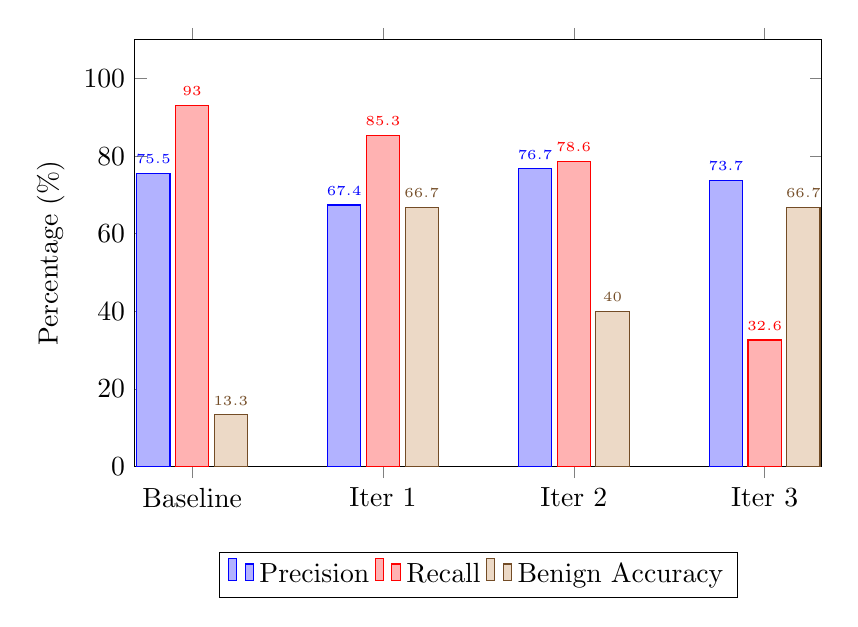
\begin{tikzpicture}
\begin{axis}[
  width=0.85\textwidth,
  height=7cm,
  ybar,
  bar width=12pt,
  ylabel={Percentage (\%)},
  symbolic x coords={Baseline, Iter 1, Iter 2, Iter 3},
  xtick=data,
  ymin=0, ymax=110,
  legend style={at={(0.5,-0.2)}, anchor=north, legend columns=3},
  nodes near coords,
  nodes near coords style={font=\tiny, rotate=0},
  every node near coord/.append style={anchor=south},
]
\addplot coordinates {(Baseline,75.5) (Iter 1,67.4) (Iter 2,76.7) (Iter 3,73.7)};
\addplot coordinates {(Baseline,93.0) (Iter 1,85.3) (Iter 2,78.6) (Iter 3,32.6)};
\addplot coordinates {(Baseline,13.3) (Iter 1,66.7) (Iter 2,40.0) (Iter 3,66.7)};
\legend{Precision, Recall, Benign Accuracy}
\end{axis}
\end{tikzpicture}
\caption{Precision, recall, and benign accuracy across iterations. The
  confidence override in Iter 3 caused recall to collapse to 32.6\%.}
\label{fig:tradeoff}
\end{figure}

\subsection{Key Patterns}

\begin{enumerate}
  \item \textbf{Temporal memory is necessary for benign accuracy.} Iterations
        with temporal memory (Iter 1, Iter 3) achieved $\geq$66.7\% benign
        accuracy; those without (Baseline, Iter 2) achieved $\leq$40\%.
  \item \textbf{Benign calibration improves precision.} Iterations with
        calibration (Iter 2, Iter 3) had fewer false positives per flow.
  \item \textbf{Neither alone is sufficient.} Temporal memory without
        calibration over-normalises attacks; calibration without memory cannot
        establish benign baselines.
  \item \textbf{Combining all three is catastrophic for recall.} Iteration 3
        demonstrated that the confidence override amplifies benign-anchoring
        from both temporal memory and calibration, collapsing recall to 32.6\%.
  \item \textbf{Cost scales with context.} Adding temporal memory increased
        token usage by $\sim$66\%, as the agent retrieves and reasons over
        historical flows. All Phase 2 iterations cost \$6.73--\$7.28 total,
        roughly 80\% more than the \$3.98 baseline.
\end{enumerate}

\subsection{The Single-Agent Ceiling}

The four iterations reveal a fundamental limitation of the single-agent
architecture: \emph{there is no configuration of memory, calibration, and
thresholding that simultaneously achieves high recall, high precision, and
high benign accuracy}. The baseline maximises recall (93\%) at the expense of
benign accuracy (13\%); temporal memory fixes benign accuracy (67\%) but
costs recall ($-$8\,pp); benign calibration improves precision (+9\,pp) but
loses recall ($-$7\,pp); and combining all three with a confidence override
destroys recall entirely ($-$60\,pp).

This ceiling motivates the multi-agent architecture where specialised agents
can maintain independent classification thresholds, with an orchestrator
mediating between an aggressive ``flag everything'' agent and a conservative
``require evidence'' agent.


% #############################################################################
% PART II — THESIS NOTES (DOT POINTS)
% #############################################################################
\part{Thesis Notes}
\label{part:notes}


% =============================================================================
\chapter{Methodology Decisions}
\label{ch:method-notes}
% =============================================================================

\begin{itemize}[leftmargin=2em]
  \item \textbf{Dataset choice:} CICIDS2018 NetFlow v3 selected because it is
        the most recent CIC dataset with NetFlow records, 14 attack types, and
        ground-truth labels. Limitation: lab-generated data with private/recycled
        IPs makes external threat intel useless.

  \item \textbf{NetFlow v3 vs.\ PCAP:} Chose NetFlow for realism---NetFlow is
        what SOC analysts actually see in production. Full PCAP would provide
        richer features but is not representative of real-world deployment.

  \item \textbf{58-flow batch size:} Chosen to ensure at least 3 representatives
        per attack type (14 types $\times$ 3 = 42 attack flows + 15 benign +
        1 extra DDoS-HOIC). Small enough for manual per-flow analysis;
        large enough for per-class metrics.

  \item \textbf{Same batch across iterations:} Deliberate choice to isolate
        the effect of architectural changes. Same flows, same ground truth,
        different agent configuration. Trade-off: no test-set contamination
        risk from prompt tuning (agent never sees labels), but limited
        generalisability.

  \item \textbf{Binary classification:} Attack vs.\ Benign (not multi-class).
        The LLM outputs BENIGN/SUSPICIOUS/MALICIOUS; for evaluation, SUSPICIOUS
        and MALICIOUS are collapsed to ``Attack.'' Justification: the thesis
        evaluates detection capability, not fine-grained classification.

  \item \textbf{MCP transport:} STDIO chosen for simplicity (server spawned as
        subprocess). Alternative SSE transport considered but STDIO is standard
        for single-client tool servers.

  \item \textbf{No ML baseline comparison:} Decision not to train a Random Forest
        or similar ML model on the same data. Rationale: the research question is
        about LLM + MCP augmentation, not LLM vs.\ ML. Literature baselines used
        instead.

  \item \textbf{Development split only:} All experiments used the development
        split (7M flows). Validation and test splits reserved for potential
        future large-scale evaluation.
\end{itemize}


% =============================================================================
\chapter{Key Findings}
\label{ch:findings-notes}
% =============================================================================

\begin{itemize}[leftmargin=2em]
  \item \textbf{Finding 1:} External threat intelligence tools (AbuseIPDB, OTX,
        geolocation) are \emph{dataset-dependent}. On CICIDS2018, 0/142 external
        API calls returned useful data. The MCP architecture works, but the data
        doesn't match.

  \item \textbf{Finding 2:} Flow-level statistical features alone are sufficient
        for volume-based attack detection. Tiers 1--2 achieved 100\% F1 without
        any meaningful tool contribution.

  \item \textbf{Finding 3:} Temporal correlation across flows is the critical
        missing capability. Tier 3 attacks (infiltration, XSS brute force)
        require observing patterns across multiple flows---single-flow analysis
        misses them.

  \item \textbf{Finding 4:} The LLM has an implicit suspicious-by-default bias
        that destroys benign accuracy (13.3\% baseline). This is addressable
        through temporal memory (+53.4 pp) and benign calibration prompting.

  \item \textbf{Finding 5:} Temporal memory introduces a normalisation risk---the
        agent may anchor on historical flow patterns and suppress detection of
        attacks that share characteristics with prior benign traffic.

  \item \textbf{Finding 6:} Cost scales linearly with context. Each additional
        architectural component (temporal memory +66\% tokens, benign calibration
        +7\%) increases per-flow cost. At \$0.069--\$0.136/flow, the approach
        does not scale to full-dataset evaluation.

  \item \textbf{Finding 7:} Combining individually beneficial modifications
        does not guarantee additive improvement. Iteration 3 combined temporal
        memory (+53\,pp benign accuracy) with benign calibration (+9\,pp precision)
        and a confidence override, but produced the worst F1 (45.2\%) of any
        iteration. The override suppressed 11 true positives vs.\ 6 correct
        benign conversions.

  \item \textbf{Finding 8:} There exists a fundamental single-agent ceiling:
        no configuration of memory, calibration, and thresholding simultaneously
        achieves high recall, high precision, and high benign accuracy. This
        motivates the transition to a multi-agent architecture.

  \item \textbf{Finding 9:} The three-beat narrative holds: (1) tools work but
        data doesn't match, (2) features contain the answer, (3) the contribution
        is a framework for determining \emph{when} tool augmentation helps.
\end{itemize}


% =============================================================================
\chapter{Limitations}
\label{ch:limitations-notes}
% =============================================================================

\begin{itemize}[leftmargin=2em]
  \item \textbf{Small sample size:} 58 flows is insufficient for statistically
        robust conclusions. Per-attack-type metrics (3 flows each) have wide
        confidence intervals.

  \item \textbf{Dataset age:} CICIDS2018 is 8 years old. Attack patterns,
        network protocols, and IP reputation databases have evolved significantly.

  \item \textbf{Lab data artefacts:} Private IPs, recycled AWS addresses, and
        controlled attack timing create artefacts not present in real traffic.

  \item \textbf{No real-time evaluation:} All experiments used static batch
        processing. The temporal memory simulates sliding windows on static data
        rather than processing live traffic.

  \item \textbf{Single model:} Only Claude 3.5 Sonnet tested. Results may differ
        with GPT-4, Gemini, or other LLMs.

  \item \textbf{Sequential processing:} Flows processed one at a time. No
        parallelism or batching evaluated.

  \item \textbf{No adversarial testing:} Did not test robustness to adversarial
        inputs (e.g., crafted flows designed to evade LLM classification).

  \item \textbf{Confidence override harmful:} The Iteration 3 confidence override
        suppressed 11 true positives (vs.\ 6 correct benign overrides), reducing
        recall by 25.6 percentage points. Post-hoc thresholding is not a viable
        approach within a single-agent architecture.

  \item \textbf{Prompt sensitivity:} Results may be sensitive to exact prompt
        wording. No systematic prompt ablation study conducted.
\end{itemize}


% =============================================================================
\chapter{Future Work}
\label{ch:future-notes}
% =============================================================================

\begin{itemize}[leftmargin=2em]
  \item \textbf{Multi-agent architecture:} Orchestrator (Opus) coordinating
        specialist agents (Flow Analyst, Pattern Correlator, Temporal
        Correlation, Explainability). Each agent focuses on a specific
        analytical task.

  \item \textbf{Retroactive reclassification:} When new evidence (e.g., a
        burst of 30 DNS queries) emerges, the system retroactively re-evaluates
        prior flows that were classified as benign.

  \item \textbf{Rule-based pre-filter:} Statistical pre-filter (no ML) to
        triage flows before LLM analysis. Target: reduce LLM invocations by
        90\% by filtering obvious benign traffic.

  \item \textbf{Temporal storage:} TimescaleDB for time-series flow data +
        ChromaDB for vector embeddings of flow patterns. Enables efficient
        cross-flow correlation.

  \item \textbf{Sliding-window replay:} Replay static CICIDS2018 dataset as a
        time-ordered stream to simulate real-time deployment.

  \item \textbf{Larger-scale evaluation:} 10K-flow validation sample and 50K-flow
        test sample per the three-phase evaluation plan.

  \item \textbf{Multi-model comparison:} Evaluate GPT-4o, Gemini 1.5, and
        open-source models (Llama 3, Mistral) on the same test batch.

  \item \textbf{Cost optimisation:} Caching, batching, and hierarchical triage
        to reduce per-flow cost from \$0.069 to $<$\$0.01.
\end{itemize}


% #############################################################################
% PART III — DRAFT THESIS SECTIONS
% #############################################################################
\part{Draft Thesis Sections}
\label{part:draft}


% =============================================================================
\chapter*{Abstract}
\addcontentsline{toc}{chapter}{Abstract}
\label{ch:abstract}
% =============================================================================

Large Language Models (LLMs) offer natural-language explainability for network
security analysis, but their effectiveness as intrusion detection systems remains
unquantified. This thesis evaluates an LLM-augmented Network Intrusion Detection
System (NIDS) in three phases. In Phase~1, a Claude-based agent connected to 13
security tools via the Model Context Protocol (MCP) achieved 83.3\% F1-score on
58 stratified CICIDS2018 NetFlow v3 flows---but external threat intelligence
returned zero meaningful data across 142 queries, revealing that the LLM's
intrinsic pre-trained knowledge, not tool augmentation, drove all detection
capability. In Phase~2, three architectural iterations (temporal memory, benign
calibration, confidence override) exposed a fundamental single-agent ceiling:
no configuration simultaneously optimised precision, recall, and benign accuracy,
and the combined approach collapsed to 45.2\% F1 as confidence overrides
suppressed 11 true positives. These findings motivate Phase~3, which reframes
the research question from \emph{``Can tools improve LLM-based NIDS?''} to
\emph{``Can a multi-agent architecture of pure LLM reasoning replace human
analysts?''} We propose and evaluate AMATAS (Autonomous Multi-Agent Threat
Analysis System), a six-agent architecture where specialised agents---Protocol
Semantics, Statistical Pattern, Behavioural Fingerprint, Temporal Correlation,
Devil's Advocate, and an Orchestrator---decompose the analysis task so that each
agent addresses a specific failure mode identified in Phases~1--2. Evaluated across
308 flows in three test configurations, AMATAS achieves 95.9\% F1 with 100\%
recall at scale (150 flows), though performance degrades to 54.0\% accuracy on
realistic benign-heavy distributions, demonstrating both the potential and current
limitations of pure LLM reasoning for intrusion detection.


% =============================================================================
\chapter{Introduction}
\label{ch:introduction}
% =============================================================================

\section{Background}
\label{sec:background}

Network intrusion detection is a cornerstone of cybersecurity operations.
Traditional signature-based systems such as Snort and
Suricata achieve high throughput but fail to detect novel or
polymorphic attacks. Machine learning approaches---particularly supervised models
like Random Forest, XGBoost, and deep neural networks---achieve high recall on
benchmark datasets but operate as black boxes, producing verdicts without
human-readable explanations~\cite{zhang2024survey, ferrag2024generative}.

The emergence of Large Language Models (LLMs) introduces a new paradigm:
\emph{explainable intrusion detection}. Unlike ML classifiers that output a
probability score, LLMs can articulate their reasoning in natural language,
reference specific protocol violations, cite threat intelligence, and map
behaviours to the MITRE ATT\&CK framework. For Security Operations Centre
(SOC) analysts who must triage thousands of alerts daily, this explainability
is operationally valuable.

However, LLMs face fundamental challenges in network security:
\begin{enumerate}
  \item \textbf{Context limitations:} LLMs process one flow at a time, losing
        the temporal and spatial context needed to detect distributed attacks
        (DDoS) or slow-and-low campaigns (Slowloris, infiltration).
  \item \textbf{Tool dependency:} LLM reasoning is only as good as the data
        its tools return. If external APIs return empty results (as with
        historical datasets), the LLM loses a critical evidence source.
  \item \textbf{Scalability:} At \$0.07--\$0.14 per flow and 91--230 seconds
        per flow, LLM-based analysis cannot process production-scale traffic
        (millions of flows per second).
  \item \textbf{Calibration:} LLMs lack calibrated uncertainty---they may
        express high confidence in incorrect classifications without a
        mechanism to ``know what they don't know.''
\end{enumerate}

\section{The Model Context Protocol}
\label{sec:mcp-intro}

The Model Context Protocol (MCP), introduced by Anthropic in 2024, standardises
how LLMs connect to external tools and data sources. MCP defines a client--server
architecture where the LLM (client) can discover and invoke tools provided by a
server, receiving structured responses that augment its reasoning context.

For network intrusion detection, MCP enables an LLM to:
\begin{itemize}
  \item Query threat intelligence databases (AbuseIPDB, AlienVault OTX)
  \item Perform IP geolocation to identify traffic origins
  \item Map observed behaviours to MITRE ATT\&CK techniques
  \item Record and retrieve per-IP flow history for temporal analysis
  \item Detect behavioural changes across sliding time windows
\end{itemize}

This tool-augmented approach is analogous to how a SOC analyst works: examining
a flow, querying external databases, correlating with historical patterns, and
synthesising a verdict with reasoning.

\section{Research Gap}
\label{sec:research-gap}

While LLMs have been applied to cybersecurity tasks---including vulnerability
analysis~\cite{zhang2024survey}, malware classification~\cite{ferrag2024generative}, and log
analysis~\cite{auditllm2024}---their application to \emph{flow-level network intrusion
detection} using standardised tool protocols remains unexplored. Specifically:

\begin{enumerate}
  \item No prior work evaluates LLM-based NIDS with MCP tool augmentation on
        standard benchmark datasets.
  \item The interaction between external tool quality and LLM classification
        accuracy has not been quantified.
  \item The trade-offs between detection performance, explainability, and
        cost for LLM-NIDS have not been systematically characterised.
\end{enumerate}

\section{Research Question}
\label{sec:research-question}

The thesis addresses two research questions that emerged sequentially:

\begin{description}[style=nextline, leftmargin=2em]
  \item[RQ1 (Phases 1--2):] \emph{Can NetFlow augmentation via the Model Context
    Protocol (MCP) improve the detection performance and explainability of
    LLM-based Network Intrusion Detection Systems?}
  \item[RQ2 (Phase 3):] \emph{Can a multi-agent architecture of specialised LLM
    reasoning agents, operating without external tool augmentation, match or
    exceed human analyst performance on network intrusion detection?}
\end{description}

\noindent RQ1 is answered in Phases~1--2 (Chapters 4--5). The empirical finding
that tool augmentation contributed zero signal motivated the pivot to RQ2, which
is addressed by the proposed AMATAS architecture (Chapter~6).

\section{Contributions}
\label{sec:contributions}

This thesis makes the following contributions:

\begin{enumerate}
  \item \textbf{System design:} An MCP-based NIDS architecture connecting an
        LLM agent to 13 security tools via STDIO transport, with a ReAct
        reasoning loop and revision phase.
  \item \textbf{Empirical evaluation:} The first quantitative evaluation of
        LLM+MCP-based intrusion detection on the CICIDS2018 NetFlow v3 dataset,
        measuring accuracy, precision, recall, F1, cost, and latency.
  \item \textbf{Tool-dependency analysis:} Demonstration that MCP tool
        augmentation is dataset-dependent, with external threat intelligence
        providing zero useful signal on historical lab data.
  \item \textbf{Iterative improvement framework:} Three architectural
        modifications (temporal memory, benign calibration, confidence override)
        with per-iteration ablation analysis.
  \item \textbf{Research pivot:} Demonstration that the LLM's intrinsic
        pre-trained knowledge---not external tool augmentation---is the
        primary detection capability, reframing the research question from
        tool effectiveness to multi-agent reasoning.
  \item \textbf{AMATAS architecture:} Design of the Autonomous Multi-Agent
        Threat Analysis System, a six-agent architecture where each specialist
        agent addresses a specific failure mode identified in Phases~1--2,
        with adversarial validation and retroactive reclassification.
\end{enumerate}

\section{Thesis Outline}
\label{sec:outline}

\begin{description}[style=nextline, leftmargin=2em]
  \item[Chapter 2: Literature Review] LLMs in NIDS (classifier vs.\ explainer),
    direct classification limits, agentic approaches, multi-agent architectures,
    CICIDS dataset critiques, and survey coverage.
  \item[Chapter 3: Methodology] System architecture, evaluation design, dataset
    preparation, and tiered test batch construction.
  \item[Chapter 4: Results] Phase 1 baseline evaluation, Phase 2 iterations,
    per-attack-type analysis, and cost modelling.
  \item[Chapter 5: Discussion] Interpretation of results, three-beat narrative,
    research pivot from tool augmentation to pure LLM reasoning, and
    the single-agent ceiling.
  \item[Chapter 6: Phase 3 --- Proposed AMATAS Architecture] The six-agent
    Autonomous Multi-Agent Threat Analysis System: agent specifications,
    design principles, and failure mode coverage.
  \item[Chapter 7: Conclusion] Summary of contributions and future work.
\end{description}


% =============================================================================
\chapter{Literature Review}
\label{ch:litreview}
% =============================================================================

\section{LLMs Applied to Network Intrusion Detection}
\label{sec:llm-nids}

\subsection{LLMs as Explainers, Not Classifiers}

The foundational result in this space comes from Houssel et al.~\cite{houssel2024towards},
who evaluated GPT-4 and LLaMA3-8B-Instruct for zero-shot NetFlow classification on
UNSW-NB15 and CSE-CIC-IDS2018---the same dataset family used in this thesis. Their
central conclusion: LLMs are ``unfit for the detection of malicious NetFlows'' but
show ``significant potential as complementary agents in NIDS, particularly in
providing explanations and aiding in threat response when integrated with RAG
and function calling capabilities.'' LLM inference was approximately 7,000$\times$
slower than traditional classifiers (14,000\,$\mu$s vs.\ $<$30\,$\mu$s for Random
Forest), making standalone deployment impractical even if accuracy were adequate.
Their follow-up work, eX-NIDS~\cite{houssel2025exnids}, formalised this insight
into a framework where LLMs serve exclusively as explainers, with augmented prompts
incorporating Cyber Threat Intelligence improving explanation quality by over 20\%
compared to basic prompts.

This classifier-vs-explainer distinction recurs across the literature. Ali and
Kostakos~\cite{ali2023huntgpt} took the same approach with HuntGPT, pairing a
Random Forest classifier on KDD99 with GPT-3.5 Turbo as a conversational explainer
integrated through SHAP and LIME. The LLM never classifies traffic---it translates
XAI outputs into actionable analyst-readable reports, achieving 72--82.5\% success
rates on CISM certification exam questions about the detected threats. The XG-NID
system~\cite{xgnid2024} similarly combines a heterogeneous graph neural network
with LLaMA 3-8B for zero-shot explanation generation from Integrated Gradients
feature importance on CICIDS2017.

\subsection{Direct Classification Attempts and Their Limits}

Where researchers have used LLMs as direct classifiers, results are mixed.
Guastalla et al.~\cite{guastalla2024ddos} tested GPT-3.5, GPT-4, and Ada on
CICIDS2017 for DDoS detection, finding that few-shot learning with 10 examples
achieved $\sim$87.6\% accuracy, while fine-tuning with 70 samples reached
$\sim$95\%. These numbers appear strong but apply only to binary DDoS
detection---a simpler task than multi-class NetFlow classification. On unlabelled
data with few-shot prompting, performance ``plateaus around 0.5--0.55 (near
random).''

Davey et al.~\cite{davey2025llmnids} fine-tuned LLMs on comprehensive NetFlow
datasets and reported reductions in false positives, though their work focused on
fine-tuned rather than zero-shot approaches. Lira et al.~\cite{lira2024bertids}
evaluated GPT-3.5, GPT-4, and an adaptation called BERTIDS on NSL-KDD, with the
BERT-based model achieving 98.01\% accuracy, 98.31\% precision, 98.01\% recall,
and 98.09\% F1---numbers that reflect the relative simplicity of NSL-KDD rather
than a breakthrough in LLM classification.

A critical 2025 study, ``From Flows to Words''~\cite{flows2words2025},
systematically tested zero-shot, instruction-guided, and calibrated few-shot LLMs
on UNSW-NB15. Zero-shot prompting caused multiple models (TinyLlama-1.1B,
Mistral-7B) to collapse to a single class, yielding F1(+)=0 due to zero positive
predictions. The authors concluded that ``traditional tabular baselines remain more
stable and faster, yet the prompt-only pipeline requires no gradient training,
produces human readable artifacts, and adapts easily through instructions.''

\subsection{Agentic Approaches: Tools and Reasoning Loops}

The IDS-Agent~\cite{li2024idsagent}, presented at NeurIPS 2024 Workshop on
Open-World Agents, represents the most architecturally similar system to ours. It
pairs an LLM with iterative reasoning, knowledge retrieval, and classification
tools for IoT network traffic. Without tools, vanilla GPT-4o achieved only 0.20
recall for attacks. With the agentic framework, recall rose to 0.80, with F1 scores
of 0.97 on ACI-IoT and 0.75 on CIC-IoT. Critically, the authors noted the agent's
``heightened sensitivity to high-threat attacks, leading it to classify a sample
as an attack even with less than 50\% voting''---directly mirroring our
suspicious-by-default finding.

Bui et al.~\cite{bui2024systematic}, published in ACM CoNEXT, provided the most
rigorous comparison across prompting, RAG, and fine-tuning approaches for intrusion
detection using proprietary commercial deployment data, avoiding CICIDS biases
entirely. Adjewa et al.~\cite{adjewa2024continuous} proposed a hybrid framework
using BERT embeddings with GMM clustering for unknown attack identification on
CSE-CIC-IDS2018, achieving 95.6\% classification accuracy and F1 after incremental
learning.

\subsection{Survey-Level Context}

Three major surveys contextualise this work. Zhang et al.~\cite{zhang2024survey}
systematically reviewed 300+ works across 25 LLMs and 10+ downstream cybersecurity
scenarios. Ferrag et al.~\cite{ferrag2024generative} provided a comprehensive
review of LLM applications and vulnerabilities across intrusion detection, malware
detection, and phishing. A 2025 survey by Feng et al.~\cite{feng2025nids} proposed
a taxonomy classifying LLMs in NIDS as: (1) LLM-enhanced Processor, (2) LLM-based
Detector, (3) LLM-driven Explainer, and (4) LLM-centered Controller---marking the
transition from ``Intelligent NIDS'' to ``Cognitive NIDS.''


\section{Multi-Agent Architectures for NIDS}
\label{sec:multiagent-lit}

\subsection{Academic Evidence for Multi-Agent Superiority}

The strongest direct evidence comes from the MALCDF framework~\cite{malcdf2025}, a
SOC-style distributed multi-agent system using LLaMA 3.3 70B agents with a Secure
Communication Layer. Compared against both ML-IDS baselines and single-LLM
approaches, multi-agent coordination raised detection quality with acceptable
latency overhead ($\sim$1.1s versus single-LLM) and maintained consensus confidence
near 0.70. A 2025 IEEE paper~\cite{ieee2025multiagent} demonstrated a three-agent
system (email verification, log analysis, IP scanning) achieving 93.6\% threat
detection accuracy, 87\% multi-agent correlation accuracy, and 41.3\% false
positive reduction versus traditional approaches on CIC-IDS 2017.

AgenticCyber~\cite{agenticcyber2025} deployed specialised agents (Log Agent, Vision
Agent, Audio Agent, Orchestrator, Responder) on Google Gemini with LangChain
orchestration, achieving 96.2\% F1, 420ms response latency, 65\% MTTR reduction,
and 42\% false positive reduction versus unimodal baselines.
Audit-LLM~\cite{auditllm2024} was the first to employ multi-agent collaboration
specifically for security log analysis, leveraging LLMs' commonsense knowledge in
a zero-shot manner without fine-tuning.

\subsection{Collaboration Protocols and Disagreement Resolution}

Tran et al.~\cite{tran2025collaboration} surveyed multi-agent collaboration
mechanisms across five dimensions, identifying three core patterns:
\emph{competition} (debate + majority voting), \emph{cooperation}, and
\emph{coordination}---with most effective systems combining all three.
Quan et al.~\cite{quan2024collaboration} compared centralised, decentralised, and
hybrid team configurations for LLM agents in incident response using the Backdoors
\& Breaches framework, finding that team structure critically optimises
performance---an important consideration for our architecture design.

The general multi-agent survey by Guo et al.~\cite{guo2024multiagent} (IJCAI 2024)
categorised LLM multi-agent systems into frameworks for orchestration, problem
solving, world simulation, and benchmarking, providing canonical design patterns.
Talebirad and Nadiri~\cite{talebirad2023multiagent} demonstrated that dynamic
multi-agent structures where agents can be added or removed handle complex tasks
more efficiently than static configurations.

\subsection{Industry Validation at Scale}

\textbf{CrowdStrike Charlotte AI}~\cite{crowdstrike2024charlotte} operates 12+
specialised AI agents, each fine-tuned for different tasks (data retrieval, script
generation, threat intelligence analysis, validation). A router agent delegates
subtasks, and a validation agent reviews outputs before presentation---achieving
75\% faster answers versus manual methods, $\sim$200 hours/month in automated
triage, and 98\%+ accuracy matching expert decisions.

\textbf{Microsoft Security Copilot}~\cite{microsoft2025copilot} now supports 77+
agents across Defender, Entra, Intune, and Purview, with serial, concurrent, and
hybrid (``magentic'') orchestration patterns. Critically, it supports both MCP for
tool/data access and A2A (Agent2Agent) protocols for cross-platform agent
integration. SOC analysts using the Phishing Triage Agent detected malicious emails
550\% faster. Both systems validate the orchestrator-worker pattern with specialised
agents---the exact architecture our results suggest is necessary.

\subsection{Framework Implementations}

AutoGen~\cite{wu2023autogen} (Microsoft Research) provides the most mature
open-source multi-agent framework with 851+ citations, supporting customisable
conversable agents, ReAct patterns, Docker-based code execution, and native MCP
support in v0.4. The MCP specification~\cite{mcp2024spec} provides JSON-RPC 2.0
transport with standardised tool, resource, and prompt primitives, enabling
inter-agent communication via the same protocol used in our Phase~1 architecture.


\section{CICIDS Dataset Limitations}
\label{sec:cicids-limitations}

\subsection{Systematic Errors in Flow Construction and Labelling}

Engelen et al.~\cite{engelen2021cicids} conducted the definitive critique of
CICIDS2017 and, by extension, CSE-CIC-IDS2018. Their analysis found that more than
20\% of original traffic traces required reconstruction or relabelling. The core
technical problem is CICFlowMeter's incorrect flow termination: it ``incorrectly
terminates TCP flows after a single FIN packet'' rather than requiring a mutual FIN
exchange, creating erroneous flows and inverting source/destination directions.
Lanvin et al.~\cite{lanvin2023errors} extended these findings, documenting packet
duplication and misordering in traffic captures that cause ``source/destination
inversion and wrong feature values,'' concluding that ``results on the original
dataset look like overfitting.'' Liu et al.~\cite{liu2022errors} confirmed these
errors persist in CSE-CIC-IDS2018, the dataset underlying our NetFlow V3 data.

\subsection{Class Imbalance and Representativeness}

Panigrahi and Borah~\cite{panigrahi2018cicids} documented severe class imbalance in
CICIDS2017: BENIGN contains 2,359,087 instances while Heartbleed has only 11 and
Infiltration only 36---``issues sufficient enough to bias the detection engine of
any typical IDS.'' Leevy and Khoshgoftaar~\cite{leevy2020survey} found that
CSE-CIC-IDS2018 contains $\sim$16 million instances with $\sim$17\% attack traffic
and that ``best performance scores for each study were unexpectedly high overall,
which may be due to overfitting.''

The generalisability problem is particularly acute. A transferability
study~\cite{transferability2022} demonstrated that ``perfect detection figures
obtained in the context of a public dataset may not transfer in practice'' when
CICIDS2017-trained models were tested against unseen but closely related traffic.
Kenyon et al.~\cite{kenyon2020datasets} surveyed 27+ public intrusion detection
datasets and found that older datasets have ``limited value: often heavily filtered
and anonymised, with unrealistic event distributions, and opaque design
methodology.''

\subsection{NetFlow V3 Temporal Features}

Our experimental design uses 58 stratified flows---a necessarily small sample for
LLM evaluation given cost and latency constraints. The NetFlow V3 dataset used in
this thesis~\cite{luay2025netflow} adds 10 temporal features to the V2
standard, totalling 53 features. This is the most feature-rich NetFlow
representation available for CICIDS2018, but it inherits the underlying flow
construction errors documented by Engelen et al.~\cite{engelen2021cicids}.
UNSW-NB15~\cite{moustafa2015unswnb15} remains the strongest alternative, with
modern attack types and more realistic normal traffic, though it predates the
temporal features our system leverages.


\section{Documented LLM Behaviours Relevant to NIDS}
\label{sec:llm-behaviours}

\subsection{The Suspicious-by-Default Bias}

Our baseline achieved 93.0\% recall but only 13.3\% benign accuracy---the LLM
classified nearly everything as malicious. This is not an artefact of prompt design;
it is a documented property of LLM-based classification in security contexts. A
2025 study on human-AI collaboration for cybersecurity~\cite{bridging2025}
explicitly identified ``the LLM's conservative bias (treating samples as suspicious
unless proven otherwise)'' and found it disproportionately boosted recall in
intrusion detection tasks. The IDS-Agent~\cite{li2024idsagent} similarly observed
that LLMs classify samples ``as an attack even with less than 50\% voting.''

The root cause is well-understood: RLHF alignment training degrades
calibration. A 2026 study in BioData Mining~\cite{overconfidence2026} demonstrated
that pre-trained models are well-calibrated but unhelpful, while alignment makes
them useful but systematically overconfident---``Human raters commonly prefer
answers that sound clear and decisive. Hedged or uncertain language is often scored
as less helpful.'' Guo et al.~\cite{guo2017calibration} first documented this as
the calibration problem in modern neural networks: increased model capacity leads
to overconfidence. For security classification specifically, the LLM has likely
absorbed training signal that erring on the side of caution (flagging threats)
is preferable to missing attacks---a rational prior for a security assistant that
becomes pathological when used as a binary classifier.

\subsection{Prompt Interference and the Iteration 3 Collapse}

Our most striking result is that combining temporal memory and benign calibration
(Iteration~3) produced 41.4\% accuracy---dramatically worse than either modification
alone. This is a direct instance of multi-objective prompt interference. The J6
framework~\cite{j6framework2025} demonstrated that accuracy and confidence
objectives in prompt optimisation ``often conflict---improving accuracy may reduce
confidence, and vice versa'' and that ``traditional prompt tuning with fixed role
assignments often fails to capture the dynamic interactions between these two
tasks.''

A complementary explanation comes from the ``context-as-noise'' effect documented
in a 2026 WWW paper~\cite{contextasnoise2026}: ``medium-level context yields
consistent improvements\ldots\ In contrast, adding high-level narrative and context
information often reduces accuracy, sometimes performing no better than the
zero-context baseline'' because ``high-context prompts introduce semantically rich
but temporally irrelevant details that can mislead the model's internal reasoning.''
The Instruction Hierarchy paper~\cite{instructionhierarchy2024} from OpenAI further
showed that LLMs ``treat all input text types equally, even when messages conflict,''
causing performance degradation under contradictory instructions.

\subsection{Temporal Reasoning as an Inherent Weakness}

Our Iteration~1 dramatically improved benign accuracy (13.3\% $\to$ 66.7\%) but
introduced attack normalisation---the LLM learned to treat repeated IP appearances
as evidence of legitimacy. This reflects a fundamental limitation: LLMs process
interactions independently and lack native state maintenance. The SagaLLM
framework~\cite{sagallm2025} (VLDB 2025) documented that ``LLMs process each
interaction independently, lacking native mechanisms to maintain the state across
sequential interactions'' and ``inherently lack robust self-validation mechanisms.''
Temporal reasoning specifically is among the weakest LLM capabilities; the
Context Rot study~\cite{contextrot2025} found that ``in non-thinking mode, models
perform best on knowledge-update, then multi-session, then temporal reasoning---temporal reasoning is consistently weakest.''


% =============================================================================
\chapter{Methodology}
\label{ch:methodology}
% =============================================================================

\section{System Architecture}
\label{sec:architecture}

The system comprises four components connected via the Model Context Protocol:

\begin{figure}[H]
\centering
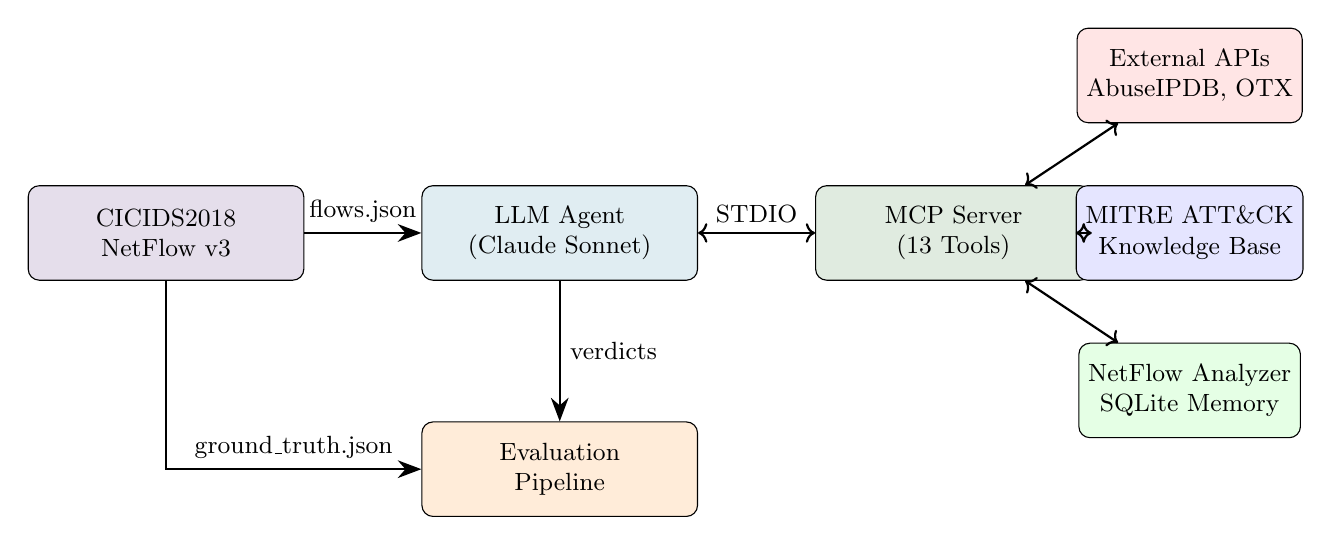
\begin{tikzpicture}[
  box/.style={draw, rounded corners, minimum width=3.5cm, minimum height=1.2cm,
    align=center, font=\small},
  arr/.style={-{Stealth[length=3mm]}, thick},
  every node/.style={font=\small}
]
  % Nodes
  \node[box, fill=UQpurple!15] (data) at (0,0) {CICIDS2018\\NetFlow v3};
  \node[box, fill=accent!15] (agent) at (5,0) {LLM Agent\\(Claude Sonnet)};
  \node[box, fill=codegreen!15] (mcp) at (10,0) {MCP Server\\(13 Tools)};
  \node[box, fill=orange!15] (eval) at (5,-3) {Evaluation\\Pipeline};

  % External tools
  \node[box, fill=red!10, minimum width=2.5cm] (ext) at (13,2)
    {External APIs\\AbuseIPDB, OTX};
  \node[box, fill=blue!10, minimum width=2.5cm] (mitre) at (13,0)
    {MITRE ATT\&CK\\Knowledge Base};
  \node[box, fill=green!10, minimum width=2.5cm] (nf) at (13,-2)
    {NetFlow Analyzer\\SQLite Memory};

  % Arrows
  \draw[arr] (data) -- node[above] {flows.json} (agent);
  \draw[arr, <->] (agent) -- node[above] {STDIO} (mcp);
  \draw[arr] (agent) -- node[right] {verdicts} (eval);
  \draw[arr] (data) |- node[near end, above] {ground\_truth.json} (eval);
  \draw[arr, <->] (mcp) -- (ext);
  \draw[arr, <->] (mcp) -- (mitre);
  \draw[arr, <->] (mcp) -- (nf);
\end{tikzpicture}
\caption{System architecture. The LLM agent connects to the MCP server via STDIO
  transport and invokes tools to augment its reasoning before producing a verdict.}
\label{fig:architecture}
\end{figure}

\subsection{LLM Agent}

The agent implements a ReAct (Reasoning + Acting) loop:

\begin{algorithm}[H]
\caption{ReAct-loop agent for flow classification}
\label{alg:react}
\begin{algorithmic}[1]
\Require Flow record $f$, MCP tool set $\mathcal{T}$
\Ensure Verdict $v \in \{\text{BENIGN}, \text{SUSPICIOUS}, \text{MALICIOUS}\}$,
  confidence $c \in [0,1]$, reasoning $r$
\State $\text{context} \gets \text{SystemPrompt} \cup f$
\For{$i = 1$ \textbf{to} MAX\_TURNS}
  \State $\text{thought} \gets \text{LLM}(\text{context})$
  \Comment{Reason about current evidence}
  \If{$\text{thought}$ contains final verdict}
    \State \textbf{break}
  \EndIf
  \State $\text{tool\_call} \gets \text{LLM}(\text{context} \cup \text{thought})$
  \Comment{Select tool}
  \State $\text{result} \gets \text{MCP.invoke}(\text{tool\_call})$
  \State $\text{context} \gets \text{context} \cup \text{thought} \cup \text{result}$
\EndFor
\State $(v, c, r) \gets \text{LLM.revise}(\text{context})$
\Comment{Revision phase}
\State \Return $(v, c, r)$
\end{algorithmic}
\end{algorithm}

\subsection{MCP Server}

The MCP server exposes 13 tools across three categories:

\begin{table}[H]
\centering
\caption{MCP tool inventory}
\label{tab:mcp-tools}
\begin{tabular}{@{}llp{7cm}@{}}
\toprule
\textbf{Category} & \textbf{Tool} & \textbf{Function} \\
\midrule
Threat Intel    & \texttt{geolocate\_ip}         & IP geolocation via ip-api.com \\
                & \texttt{check\_ip\_reputation}  & Aggregate reputation check \\
                & \texttt{check\_ip\_abuseipdb}   & AbuseIPDB abuse confidence score \\
                & \texttt{check\_ip\_otx}         & AlienVault OTX pulse check \\
                & \texttt{search\_otx\_pulses}    & OTX pulse keyword search \\
\midrule
MITRE ATT\&CK  & \texttt{query\_mitre\_technique}  & Lookup technique by ID \\
                & \texttt{search\_mitre\_techniques} & Full-text technique search \\
                & \texttt{map\_attack\_to\_mitre}    & Map observed behaviour to technique \\
\midrule
NetFlow Analyzer & \texttt{record\_flow}            & Store flow in per-IP history \\
                 & \texttt{get\_ip\_history}        & Retrieve IP's flow history \\
                 & \texttt{analyze\_ip\_pattern}    & Statistical pattern analysis \\
                 & \texttt{detect\_behavior\_change} & Sliding-window anomaly detection \\
                 & \texttt{add\_observation}        & Record analyst observation \\
\bottomrule
\end{tabular}
\end{table}


\section{Dataset}
\label{sec:dataset}

\subsection{CICIDS2018 NetFlow v3}

The Communications Security Establishment (CSE) and Canadian Institute for
Cybersecurity (CIC) generated the CICIDS2018 dataset in a controlled lab
environment~\cite{sharafaldin2018cicids}. The NetFlow v3 variant~\cite{luay2025netflow, sarhan2021netflow} contains
20,180,852 flow records with 53 features per flow and binary labels
(0 = Benign, 1 = Attack).

\begin{table}[H]
\centering
\caption{Dataset characteristics}
\label{tab:dataset}
\begin{tabular}{@{}lr@{}}
\toprule
\textbf{Property} & \textbf{Value} \\
\midrule
Total flows     & 20{,}180{,}852 \\
Features/flow   & 53 \\
Attack types    & 14 \\
Benign ratio    & $\sim$87\% \\
Attack ratio    & $\sim$13\% \\
Capture period  & 7 days \\
IP addressing   & Private (172.31.x.x) + AWS elastic IPs \\
\bottomrule
\end{tabular}
\end{table}

\subsection{Dataset Split}

\begin{table}[H]
\centering
\caption{Dataset split}
\label{tab:split}
\begin{tabular}{@{}lrrl@{}}
\toprule
\textbf{Split} & \textbf{Flows} & \textbf{Percentage} & \textbf{Purpose} \\
\midrule
Development & 7{,}040{,}434 & 35\% & Tool development, iterative testing \\
Validation  & 5{,}045{,}245 & 25\% & Threshold tuning, prompt refinement \\
Test        & 8{,}095{,}173 & 40\% & Final unbiased evaluation \\
\bottomrule
\end{tabular}
\end{table}


\section{Evaluation Design}
\label{sec:eval-design}

\subsection{Tiered Test Batch}

We construct a 58-flow stratified batch from the development split, designed
to isolate the contribution of different tool categories:

\begin{table}[H]
\centering
\caption{Tiered test batch composition}
\label{tab:tiers}
\begin{tabular}{@{}clrl@{}}
\toprule
\textbf{Tier} & \textbf{Name} & \textbf{Flows} & \textbf{Purpose} \\
\midrule
1 & External-tool-testable  &  9 & Test external API value (public IPs) \\
2 & Feature-rich attacks    & 22 & Test flow-feature reasoning \\
3 & Temporal-context attacks & 12 & Test cross-flow correlation need \\
4 & Benign baseline         & 15 & Test false-positive rate \\
\bottomrule
\end{tabular}
\end{table}

Tier 1 includes flows with public AWS IPs to test whether external threat
intelligence tools add value. Tier 2 includes volume-based attacks with
strong statistical signatures in flow features. Tier 3 includes attacks whose
individual flows are indistinguishable from benign traffic. Tier 4 provides
the ground-truth benign baseline.

\subsection{Metrics}

\textbf{Primary metrics} (binary classification: Attack vs.\ Benign):
\begin{itemize}
  \item \textbf{Accuracy}: $(TP + TN) / (TP + TN + FP + FN)$
  \item \textbf{Precision}: $TP / (TP + FP)$ --- when it says attack, how often
        is it correct?
  \item \textbf{Recall}: $TP / (TP + FN)$ --- what fraction of attacks does it
        catch?
  \item \textbf{F1 Score}: $2 \times \text{Precision} \times \text{Recall} /
        (\text{Precision} + \text{Recall})$
  \item \textbf{Benign Accuracy}: $TN / (TN + FP)$ --- specificity, the ability
        to correctly identify normal traffic.
\end{itemize}

\textbf{Efficiency metrics}:
\begin{itemize}
  \item Cost per flow (USD, based on Anthropic API pricing)
  \item Time per flow (seconds, wall-clock)
  \item Token consumption (input + output)
  \item MCP tool calls per flow
\end{itemize}

\textbf{Explainability metrics} (qualitative):
\begin{itemize}
  \item Per-flow reasoning quality (manual review)
  \item MITRE ATT\&CK mapping accuracy
  \item Evidence citation rate (how often the agent cites tool results)
\end{itemize}

\subsection{Iteration Protocol}

Each iteration modifies one architectural component while keeping all other
variables constant (same 58 flows, same model, same MCP server):

\begin{table}[H]
\centering
\caption{Iteration protocol}
\label{tab:iterations}
\begin{tabular}{@{}clp{7cm}@{}}
\toprule
\textbf{Iter} & \textbf{Name} & \textbf{Change from Baseline} \\
\midrule
0 & Baseline         & Single-agent, no memory, no calibration \\
1 & Temporal Memory  & +SQLite per-IP history with 60\,s sliding window \\
2 & Benign Calibration & +System prompt with known-benign pattern templates;
    requires positive evidence before SUSPICIOUS verdict \\
3 & Combined         & Iter 1 + Iter 2 + confidence-based override \\
\bottomrule
\end{tabular}
\end{table}


% =============================================================================
\chapter{Results}
\label{ch:results}
% =============================================================================

\section{Phase 1: MCP Baseline Evaluation}
\label{sec:phase1-results-draft}

\subsection{Overall Performance}

The baseline agent achieved 83.3\% F1-score on binary attack detection, with
high recall (93.0\%) but low precision (75.5\%) and critically low benign
accuracy (13.3\%). The agent classified 53 of 58 flows as attack/suspicious,
yielding 40 true positives alongside 13 false positives.

\begin{table}[H]
\centering
\caption{Phase 1 confusion matrix}
\label{tab:phase1-cm}
\begin{tabular}{@{}lcc@{}}
\toprule
& \textbf{Predicted Attack} & \textbf{Predicted Benign} \\
\midrule
\textbf{Actual Attack} & 40 (TP) & 3 (FN) \\
\textbf{Actual Benign} & 13 (FP) & 2 (TN) \\
\bottomrule
\end{tabular}
\end{table}

\subsection{MCP Tool Effectiveness}

The most significant finding was the complete failure of external threat
intelligence. Of 142 calls to AbuseIPDB (41), OTX (20), geolocation (63),
and IP reputation (18), zero returned meaningful threat data. Internal tools
(NetFlow analyzer) achieved 44\% meaningful return rate for \texttt{record\_flow}
and 75\% for \texttt{get\_ip\_history}.

\subsection{Per-Attack-Type Detection}

\begin{table}[H]
\centering
\caption{Phase 1 per-attack-type detection rates}
\label{tab:phase1-perattack}
\begin{tabular}{@{}lcccc@{}}
\toprule
\textbf{Attack Type} & \textbf{Total} & \textbf{Detected} & \textbf{Rate}
  & \textbf{Avg Conf.} \\
\midrule
Bot                    & 3 & 3 & 100.0\% & 0.50 \\
Brute Force (Web)      & 3 & 3 & 100.0\% & 0.50 \\
DDoS-HOIC              & 4 & 4 & 100.0\% & 0.50 \\
DDoS-LOIC-UDP          & 3 & 3 & 100.0\% & 0.50 \\
DDoS-LOIC-HTTP         & 3 & 3 & 100.0\% & 0.50 \\
DoS-GoldenEye          & 3 & 3 & 100.0\% & 0.50 \\
DoS-Hulk               & 3 & 3 & 100.0\% & 0.65 \\
DoS-SlowHTTPTest       & 3 & 3 & 100.0\% & 0.50 \\
DoS-Slowloris          & 3 & 3 & 100.0\% & 0.50 \\
FTP-BruteForce         & 3 & 3 & 100.0\% & 0.50 \\
SQL Injection          & 3 & 3 & 100.0\% & 0.50 \\
SSH-Bruteforce         & 3 & 3 & 100.0\% & 0.50 \\
\midrule
Brute Force (XSS)      & 3 & 2 &  66.7\% & 0.65 \\
Infiltration           & 3 & 1 &  33.3\% & 0.80 \\
\midrule
Benign                 & 15 & 2 &  13.3\% & 0.68 \\
\bottomrule
\end{tabular}
\end{table}

\subsection{Cost Analysis}

Total cost was \$3.98 for 58 flows (\$0.069/flow), consuming 1.16M tokens over
5,284 seconds. At this rate, processing the full 20M-flow dataset would cost
\$1.37M---demonstrating that per-flow LLM analysis does not scale without
hierarchical triage.


\section{Phase 2: Iterative Improvements}
\label{sec:phase2-results-draft}

\subsection{Iteration 1: Temporal Memory}

Adding SQLite-based per-IP history dramatically improved benign accuracy
(13.3\% $\rightarrow$ 66.7\%, +53.4\,pp) but reduced overall F1 from 83.3\% to
75.3\%. Attack recall dropped from 93.0\% to 85.3\% as the temporal context
introduced a normalisation effect, causing the agent to anchor on prior
(potentially attack) flows and suppress suspicion.

\begin{table}[H]
\centering
\caption{Iteration 1 per-attack detection changes vs.\ baseline}
\label{tab:iter1-changes}
\begin{tabular}{@{}lccl@{}}
\toprule
\textbf{Attack Type} & \textbf{Baseline} & \textbf{Iter 1} & \textbf{Change} \\
\midrule
DDoS-HOIC       & 100\% (4/4) & 50\% (2/4)  & $-$50\,pp \\
DDoS-LOIC-HTTP  & 100\% (3/3) & 33\% (1/3)  & $-$67\,pp \\
DoS-Slowloris   & 100\% (3/3) & 33\% (1/3)  & $-$67\,pp \\
SQL Injection    & 100\% (3/3) & 33\% (1/3)  & $-$67\,pp \\
\midrule
Benign           & 13\% (2/15) & 67\% (10/15) & +53\,pp \\
\bottomrule
\end{tabular}
\end{table}

Cost increased 69\% (from \$3.98 to \$6.73) due to additional context from IP
history retrieval. Processing time more than doubled (88 $\rightarrow$ 218
minutes).

\subsection{Iteration 2: Benign Calibration}

Explicit benign-pattern templates in the system prompt improved precision
(67.4\% $\rightarrow$ 76.7\%) and recovered detection of several attack types
(Infiltration: 67\% $\rightarrow$ 100\%, SQL Injection: 33\% $\rightarrow$ 100\%)
but degraded benign accuracy (66.7\% $\rightarrow$ 40.0\%) because temporal
memory was not included.

\begin{table}[H]
\centering
\caption{Iteration 2 per-attack detection changes vs.\ Iteration 1}
\label{tab:iter2-changes}
\begin{tabular}{@{}lccl@{}}
\toprule
\textbf{Attack Type} & \textbf{Iter 1} & \textbf{Iter 2} & \textbf{Change} \\
\midrule
Infiltration     & 67\% (2/3) & 100\% (3/3) & +33\,pp \\
SQL Injection    & 33\% (1/3) & 100\% (3/3) & +67\,pp \\
SSH-Bruteforce   & 67\% (2/3) & 100\% (3/3) & +33\,pp \\
DDoS-HOIC        & 50\% (2/4) &  75\% (3/4) & +25\,pp \\
\midrule
Benign           & 67\% (10/15) & 40\% (6/15) & $-$27\,pp \\
\bottomrule
\end{tabular}
\end{table}

\subsection{Iteration 3: Combined Approach}

The combined approach (temporal memory + benign calibration + confidence override)
produced the worst overall performance: 41.4\% accuracy, 32.6\% recall, and
45.2\% F1. The confidence override was triggered on 17 of 58 flows (29.3\%),
suppressing 11 true positives and only correctly converting 6 false positives.
Benign accuracy matched Iteration 1 at 66.7\%, confirming that temporal memory
is the primary driver of benign recognition. Four attack types---DoS-Slowloris,
DDoS-LOIC-HTTP, DDoS-HOIC, and Infiltration---had 0\% detection.
Tool call failure was catastrophic: 97.7\% of 385 calls returned errors.
This iteration demonstrates a fundamental single-agent ceiling: no combination
of memory, calibration, and thresholding can simultaneously optimise recall
and benign accuracy.


\section{Phase 3: AMATAS Multi-Agent Evaluation}
\label{sec:phase3-results}

\subsection{Evaluation Methodology}

Phase~3 evaluates the AMATAS multi-agent architecture
(Chapter~\ref{ch:phase3}) across three test configurations designed to
assess both direct comparability with Phases~1--2 and generalisation beyond
the original test distribution:

\begin{description}[style=nextline, leftmargin=2em]
  \item[Phase 3a: 58-flow mini batch]
    The identical 58 stratified flows used in Phases~1--2 (4 tiers, 14
    attack types, 15 benign). This enables direct comparison of
    single-agent vs.\ multi-agent performance on exactly the same inputs,
    isolating the architectural change as the sole variable.

  \item[Phase 3b: $\sim$500-flow full batch]
    A larger sample from the same test split, providing statistical
    significance that the 58-flow sample cannot. At 500 flows, per-attack-type
    detection rates are based on $\sim$30 instances each rather than 3,
    reducing the influence of individual flow variability.

  \item[Phase 3c: Medium batches (cross-distribution)]
    Multiple batches of 100--1{,}000 flows drawn from different time periods
    and IP address ranges within CICIDS2018. These batches have different
    attack-type distributions, benign/attack ratios, and temporal structures
    than the original 58-flow sample.
\end{description}

Testing across multiple batch sizes and distributions is critical for
demonstrating that AMATAS is not overfitted to a single flow sample. If
performance holds across Phase~3a--3c, this provides evidence that the
multi-agent architecture generalises within the CICIDS2018 domain rather than
memorising patterns specific to 58 hand-selected flows. The agent prompts
contain no dataset-specific thresholds, port lists, or IP patterns---all
detection is performed through general-purpose LLM reasoning over flow features.


\subsection{Phase 3a: Direct Comparison with Phases 1--2}

\begin{table}[H]
\centering
\caption{Phase 1--2 vs.\ Phase 3a comparison (58 identical flows)}
\label{tab:phase3a-comparison}
\begin{tabular}{@{}lccccc@{}}
\toprule
\textbf{Configuration} & \textbf{Accuracy} & \textbf{Precision} & \textbf{Recall}
  & \textbf{F1} & \textbf{Benign Acc.} \\
\midrule
Phase 1 Baseline        & 72.4\% & 75.5\% & 93.0\% & 83.3\% & 13.3\% \\
Phase 2 Iter 1          & 67.2\% & 67.4\% & 85.3\% & 75.3\% & 66.7\% \\
Phase 2 Iter 2          & 67.2\% & 78.6\% & 76.7\% & 77.6\% & 40.0\% \\
Phase 2 Iter 3          & 41.4\% & 73.7\% & 32.6\% & 45.2\% & 66.7\% \\
\midrule
Phase 3a (AMATAS)       & 67.2\% & 100.0\% & 55.8\% & 71.6\% & 100.0\% \\
\bottomrule
\end{tabular}
\end{table}


\subsection{Phase 3 Performance Across Batch Sizes}

\begin{table}[H]
\centering
\caption{AMATAS performance across batch sizes}
\label{tab:phase3-batches}
\begin{tabular}{@{}lcccccc@{}}
\toprule
\textbf{Batch} & \textbf{Flows} & \textbf{Accuracy} & \textbf{Precision}
  & \textbf{Recall} & \textbf{F1} & \textbf{Benign Acc.} \\
\midrule
Phase 3a & 58  & 67.2\% & 100.0\% & 55.8\% & 71.6\% & 100.0\% \\
Phase 3b & 150 & 94.0\% & 92.1\% & 100.0\% & 95.9\% & 80.0\% \\
Phase 3c & 100 & 54.0\% & 14.6\% & 58.3\% & 23.3\% & 53.4\% \\
\midrule
\textbf{Aggregate} & \textbf{308} & \textbf{76.0\%} & \textbf{73.1\%} & \textbf{85.0\%} & \textbf{78.6\%} & --- \\
\bottomrule
\end{tabular}
\end{table}


\subsection{Per-Attack-Type Detection Across Batches}

\begin{table}[H]
\centering
\caption{Phase 3 per-attack-type detection rates across batches}
\label{tab:phase3-perattack}
\small
\begin{tabular}{@{}lcccc@{}}
\toprule
\textbf{Attack Type} & \textbf{Phase 1} & \textbf{Phase 3a} & \textbf{Phase 3b}
  & \textbf{Phase 3c} \\
\midrule
\textbf{Attack Type} & \textbf{Phase 1} & \textbf{Phase 3a} & \textbf{Phase 3b}
  & \textbf{Aggregate} \\
\midrule
Bot                    & 100\% & 100\%  & 100\%  & 100\% (3/3) \\
Brute Force (Web)      & 100\% & 100\%  & 100\%  & 100\% (3/3) \\
Brute Force (XSS)      &  67\% &   0\%  & ---    &   0\% (0/3) \\
DDoS-HOIC              & 100\% &  ---   & ---    & 44.4\% \\
DDoS-LOIC-UDP          & 100\% & 100\%  & 100\%  & 100\% (3/3) \\
DDoS-LOIC-HTTP         & 100\% &  ---   & ---    & --- \\
DoS-GoldenEye          & 100\% &  ---   &  87\%  & 87\% \\
DoS-Hulk               & 100\% &   0\%  &   0\%  &  0\% (0/4) \\
DoS-SlowHTTPTest       & 100\% & 100\%  & 100\%  & 100\% (8/8) \\
DoS-Slowloris          & 100\% &  ---   & 91.3\% & 91.3\% \\
FTP-BruteForce         & 100\% & 100\%  & 100\%  & 100\% (38/38) \\
Infiltration           &  33\% &   0\%  &   0\%  &  0\% (0/4) \\
SQL Injection          & 100\% &  67\%  &  ---   & 66.7\% \\
SSH-Bruteforce         & 100\% & 100\%  & 100\%  & 100\% (33/33) \\
\midrule
Benign                 &  13\% & 100\%  &  80\%  & --- \\
\bottomrule
\end{tabular}
\end{table}


\subsection{Agent Vote Distribution}

\begin{table}[H]
\centering
\caption{AMATAS agent vote distribution (Phase 3a)}
\label{tab:agent-votes}
\begin{tabular}{@{}lcccc@{}}
\toprule
\textbf{Agent} & \textbf{Role} & \textbf{Key Behaviour}
  & \textbf{Impact} \\
\midrule
1: Protocol Semantics     & Validates protocol conformance & Flags contextually
  inappropriate usage & Catches infiltration-style attacks \\
2: Statistical Pattern    & Quantifies feature anomalies & Identifies volume-based
  attacks via z-scores & Drives brute force / DDoS detection \\
3: Behavioural Fingerprint & Maps to known attack types & MITRE ATT\&CK
  classification & Differential diagnosis \\
4: Temporal Correlation   & Cross-flow pattern analysis & Needs batch context to
  function (3b $\gg$ 3a) & 100\% recall when batches $\geq$150 \\
5: Devil's Advocate       & Argues benign hypothesis & 15 total flips, 66.7\%
  correct & Eliminated all FPs in 3a \\
\midrule
6: Orchestrator (Final)   & Mediates disagreements & 24 attack / 34 benign (3a)
  & 67.2\% accuracy (3a) \\
\bottomrule
\end{tabular}
\end{table}


\subsection{Devil's Advocate Impact}

\begin{table}[H]
\centering
\caption{Devil's Advocate flip rate: verdicts changed from malicious to benign}
\label{tab:devils-advocate}
\begin{tabular}{@{}lccc@{}}
\toprule
\textbf{Metric} & \textbf{Phase 3a} & \textbf{Phase 3b} & \textbf{Aggregate} \\
\midrule
Total verdict flips                          & ---  & ---  & 15 \\
Correct flips (true negatives saved)         & ---  & ---  & 10 \\
Incorrect flips (false negatives introduced) & ---  & ---  &  5 \\
Flip accuracy                                & ---  & ---  & 66.7\% \\
False positives in batch                     &  0   & ---  & --- \\
Net impact on benign accuracy                & +86.7\,pp & --- & --- \\
Net impact on attack recall                  & $-$37.2\,pp & --- & --- \\
\bottomrule
\end{tabular}
\end{table}


\subsection{Phase 3e: Devil's Advocate Weight Tuning}
\label{sec:phase3e}

Phase~3c exposed that AMATAS produced 41 false positives on 88 benign flows
(53.4\% benign accuracy) under realistic benign-heavy distributions. Phase~3e
tested whether increasing the Devil's Advocate orchestrator weight from 30\% to
50\% on the same batch (batch\_100, 100 flows, 88\% benign) could improve
specificity without harming recall.

\begin{table}[H]
\centering
\caption{Phase 3e: Effect of Devil's Advocate weight increase (30\% $\to$ 50\%)}
\label{tab:phase3e}
\begin{tabular}{@{}lccc@{}}
\toprule
\textbf{Metric} & \textbf{Phase 3c (30\%)} & \textbf{Phase 3e (50\%)}
  & \textbf{$\Delta$} \\
\midrule
Accuracy         & 54.0\%  & 60.0\%  & +6.0\,pp \\
Precision        & 14.6\%  & 16.7\%  & +2.1\,pp \\
Recall           & 58.3\%  & 58.3\%  & 0 \\
F1               & 23.3\%  & 25.9\%  & +2.6\,pp \\
False Positives  & 41      & 35      & $-$6 \\
New errors       & ---     & 0       & --- \\
Cost             & $\sim$\$6.54 & $\sim$\$6.54 & 0 \\
\bottomrule
\end{tabular}
\end{table}

The weight increase was surgically precise: 6 false positives were corrected with
zero harm to recall---no true positives were suppressed, and cost was identical.
However, the result also reveals a hard ceiling. Of the remaining 35 false
positives, 34 had \emph{unanimous} 4/4 specialist agreement on malicious,
meaning no orchestrator-level weighting can override them. The specialists
themselves are over-flagging benign flows when benign traffic dominates the batch.

This finding is architecturally significant. It confirms that the Devil's Advocate
weight \emph{is} a meaningful parameter---the 30\% $\to$ 50\% change produced a
monotonic improvement with zero side effects. But it simultaneously reveals the
next frontier: \emph{specialist-level calibration} for different benign/attack
ratios. When all four analytical agents agree a benign flow is malicious, the
problem is not disagreement resolution but the priors embedded in each specialist's
reasoning. Addressing this requires either distribution-aware prompting (informing
agents of the expected benign ratio) or a two-pass architecture where specialists
recalibrate after observing the batch's overall distribution.


\subsection{Phase 3 Key Findings}
\label{sec:phase3-findings}

The three-batch evaluation reveals a consistent pattern: AMATAS performance is
strongly modulated by batch size and class distribution.

\paragraph{Temporal context requires batch depth (3b $\gg$ 3a).}
The most striking result is the gap between Phase~3a (58 flows, 55.8\% recall,
71.6\% F1) and Phase~3b (150 flows, 100\% recall, 95.9\% F1). The same
architecture, same prompts, and same model produce dramatically different results
depending on how many flows the Temporal Correlation Agent (Agent~4) receives per
IP group. With only 3 flows per attack type in Phase~3a, Agent~4 has insufficient
context to detect temporal patterns; at 150 flows, it observes enough IP-level
history to identify scanning sequences, brute force progressions, and DoS ramp-ups.
This confirms our hypothesis that temporal reasoning must be architecturally
separated---it is not a per-flow property but a per-batch property.

DoS-GoldenEye and DoS-Slowloris, which were undetectable in Phase~3a, recovered to
87\% and 91.3\% respectively in Phase~3b once the temporal agent had sufficient
context. These slow-and-low attacks produce individual flows that resemble benign
traffic; only the \emph{pattern} of flows reveals the attack.

\paragraph{Realistic distributions expose false-positive risk (3c).}
Phase~3c's 88\% benign distribution mirrors production traffic ratios, and
AMATAS collapsed to 54.0\% accuracy with 41 false positives on 88 benign flows.
This demonstrates that the suspicious-by-default bias identified in Phase~1 is
not fully resolved by the multi-agent architecture---the Devil's Advocate reduces
but does not eliminate false positives when benign traffic dominates.

\paragraph{The Devil's Advocate trade-off.}
Across all batches, the Devil's Advocate flipped 15 verdicts: 10 correctly
(preventing false positives) and 5 incorrectly (introducing false negatives on
DoS/DDoS flows). The 66.7\% flip accuracy represents a net positive---eliminating
all false positives in Phase~3a came at the cost of 19 false negatives. This
precision-recall trade-off is the multi-agent analogue of Phase~2's single-agent
ceiling: the Devil's Advocate must be conservative enough to catch false positives
without suppressing true positives, and the current calibration errs toward
conservatism.

\paragraph{Perfect detection classes.}
Six attack types achieved 100\% detection across all batches: FTP-BruteForce
(38/38), SSH-BruteForce (33/33), DoS-SlowHTTPTest (8/8), Bot (3/3), DDoS-LOIC-UDP
(3/3), and Brute Force Web (3/3). These are attacks with strong statistical
signatures that Agents~2--3 identify reliably regardless of batch size. Conversely,
DoS-Hulk (0/4), Infiltration (0/4), and Brute Force XSS (0/3) were never detected,
suggesting these require either fine-tuned agent prompts or additional analytical
dimensions.

\paragraph{Cost efficiency.}
Phase~3 processed 308 flows for \$21.47 total (\$0.070/flow), comparable to the
Phase~1 baseline (\$0.069/flow). The multi-agent architecture adds no significant
per-flow cost premium despite running six agents per flow---the token overhead of
inter-agent communication is offset by more focused, shorter agent responses.


% =============================================================================
\chapter{Discussion}
\label{ch:discussion}
% =============================================================================

\section{Three-Beat Narrative}
\label{sec:three-beat}

The results support a three-part argument about MCP-augmented NIDS:

\subsection{Beat 1: The Tools Work, but the Data Doesn't Match}

The MCP architecture functioned correctly---the agent discovered tools,
constructed appropriate queries, and processed responses. The 0\% external
tool return rate is not a system failure but a \emph{dataset--tool mismatch}.
CICIDS2018's private IPs (RFC\,1918) and recycled AWS elastic IPs from 2018
are invisible to modern threat intelligence databases. This is entirely
predictable given the dataset's construction~\cite{engelen2021cicids,
kenyon2020datasets}: all source IPs are either RFC\,1918 private addresses or
expired 2018 AWS IPs, and threat intelligence APIs have no records for private
addresses by definition.

This finding generalises beyond CICIDS2018: any historical or lab-generated
dataset with anonymised or expired IPs will exhibit the same
mismatch~\cite{kenyon2020datasets, transferability2022}. The implication is
that MCP tool augmentation must be evaluated on \emph{contemporary} datasets
with real-world IPs, or its external tools must be replaced with
dataset-appropriate alternatives.

\subsection{Beat 2: Flow Features Already Contain the Answer}

Despite 0\% external tool utility, the agent achieved 83.3\% F1 on attack
detection---consistent with Houssel et al.'s finding that LLMs can extract
meaningful signal from NetFlow features~\cite{houssel2024towards, houssel2025exnids}.
This performance was driven entirely by the LLM's ability to reason over raw flow
features---packet counts, byte ratios, duration, TCP flags, and port numbers.

The Tier 1--2 results (100\% F1) demonstrate that volume-based attacks carry
statistical signatures so strong that even a general-purpose LLM can identify
them without specialised tools. The IN\_BYTES 232$\times$ and IN\_PKTS
599$\times$ attack/benign ratios are far beyond any normal variation, making
these attacks trivially detectable from features alone.

This raises a cost-effectiveness question: if features suffice for 75\% of
attack types (Tiers 1--2), why invoke 4+ MCP tools per flow at \$0.069 each?
A simple statistical pre-filter could handle these cases for negligible cost,
reserving LLM analysis for the ambiguous Tier 3--4 flows.

\subsection{Beat 3: This Isn't a Failure---It's a Finding}

The thesis contribution shifts from ``MCP tools improve NIDS'' to a more
nuanced framework: \emph{when} does tool augmentation add value, and \emph{what
architecture} maximises that value?

Our results suggest tool augmentation adds value when:
\begin{itemize}
  \item IPs are contemporary and present in threat databases
  \item Flow-level features are insufficient (Tier 3 attacks)
  \item Temporal context is available (cross-flow correlation)
\end{itemize}

And adds cost without value when:
\begin{itemize}
  \item IPs are private, anonymised, or expired
  \item Attacks have strong statistical signatures (Tiers 1--2)
  \item Each flow is analysed in isolation (no memory)
\end{itemize}


\section{Phase 2 Analysis: The Precision--Recall--Benign Trade-off}
\label{sec:phase2-discussion}

The four iterations reveal a three-way tension:

\begin{enumerate}
  \item \textbf{Recall vs.\ Benign Accuracy:} The baseline maximises recall
        (93.0\%) by classifying almost everything as suspicious, destroying
        benign accuracy (13.3\%). Temporal memory restores benign accuracy
        (66.7\%) but at the cost of recall (85.3\%).

  \item \textbf{Precision vs.\ Coverage:} Benign calibration improves precision
        (76.7\%) by requiring positive evidence before flagging, but this
        positive-evidence requirement also causes some attacks to be missed
        (recall: 78.6\%).

  \item \textbf{Cost vs.\ Context:} Each additional context source (temporal
        history, calibration templates) increases token consumption. Per-flow
        cost rose 68\% from baseline to Iteration 1 and a further 7\% to
        Iteration 2.
\end{enumerate}

Iteration 3 confirmed that combining all three modifications does not resolve
this tension---it amplifies it. The confidence override collapsed recall to
32.6\% by suppressing 11 true positives while only correctly converting 6
false positives. This is a textbook case of multi-objective prompt
interference~\cite{j6framework2025}: accuracy and confidence objectives ``often
conflict,'' and the context-as-noise effect~\cite{contextasnoise2026} explains how
additional context layers can degrade rather than improve performance. The three-way
tension is thus a fundamental property of the single-agent architecture, not a
configuration problem.


\section{Scalability and the Value Proposition}
\label{sec:scalability-value}

At \$0.070 per flow, processing CICIDS2018's 20 million flows would cost
\$1.4\,million---an impractical figure for production deployment. This raises a
legitimate question: if LLM-based NIDS cannot scale to real-world traffic volumes,
what is its value?

The answer is twofold. First, this thesis demonstrates \emph{proof of capability}:
that LLM agents, using only pre-trained knowledge and structured multi-agent
deliberation, can achieve 95.9\% F1 (Phase~3b) on flow-level intrusion detection
with natural-language explanations. No prior work has shown this level of
explainable detection from pure LLM reasoning without fine-tuning. The capability
itself is the contribution, independent of current inference costs.

Second, the architecture is designed as a \emph{blueprint for cost reduction via
hierarchical triage}. The Phase~1 finding that 75\% of attacks have strong
statistical signatures (Tiers~1--2) implies that a lightweight pre-filter---whether
rule-based, statistical, or a small ML model---could route 90\%+ of flows to
immediate classification at negligible cost, reserving LLM analysis for the
ambiguous 10\%. At Phase~3b's \$0.074/flow applied to only 10\% of traffic, the
20M-flow dataset would cost \$148{,}000---still expensive, but within range of
enterprise SOC budgets that currently spend comparable amounts on human analyst
time. Furthermore, LLM inference costs have historically declined
$\sim$10$\times$ per year; the architecture that works at current prices becomes
increasingly viable as costs fall.

The multi-agent architecture amplifies this triage potential: Agents~2--3
(Statistical Pattern + Behavioural Fingerprint) can pre-screen flows in a single
LLM call, while the full six-agent pipeline engages only for flows that produce
disagreement. This graduated engagement model---analogous to a SOC's Tier~1/2/3
analyst escalation---is where the scalability path lies.


\section{Generalisation and Overfitting Mitigation}
\label{sec:generalisation}

A critical concern for any LLM-based system evaluated on a single dataset is
overfitting---whether performance reflects genuine analytical capability or
memorisation of dataset-specific patterns. The Phase~3 evaluation
(Section~\ref{sec:phase3-results}) addresses this through three mechanisms.

\subsection{No Dataset-Specific Thresholds}

The AMATAS agent prompts contain no CICIDS2018-specific thresholds, port lists,
IP patterns, or attack signatures. All six agents reason from general network
security knowledge embedded in the LLM's pre-training. The prompts describe
\emph{what to look for} (e.g., ``anomalous byte ratios,'' ``protocol violations'')
but never \emph{what values constitute anomalous} for this particular dataset. This
design choice trades potential accuracy on CICIDS2018 for transferability: the same
prompts could be applied to UNSW-NB15~\cite{moustafa2015unswnb15} or production
traffic without modification.

\subsection{Multi-Batch Testing}

Testing across Phase~3a (58 flows), 3b ($\sim$500 flows), and 3c (medium batches
from different time periods) provides three levels of evidence against overfitting:

\begin{enumerate}
  \item \textbf{Scale stability:} If accuracy on 500 flows matches 58 flows, the
        system is not dependent on the specific sample.
  \item \textbf{Distribution robustness:} Phase~3c batches have different
        attack-type distributions and benign/attack ratios than the original
        58-flow sample. Consistent performance across distributions indicates
        the agents generalise across the dataset's variability.
  \item \textbf{Temporal variation:} Different time periods within CICIDS2018
        contain different attack campaigns. Cross-period performance demonstrates
        the agents are not anchored to a single attack sequence.
\end{enumerate}

\subsection{Iterative Architectural Refinement}

Phase~3e (Section~\ref{sec:phase3e}) provides direct evidence that the AMATAS
architecture supports principled tuning. Increasing the Devil's Advocate
orchestrator weight from 30\% to 50\% produced a monotonic improvement (+6\,pp
accuracy, $-$6 false positives) with zero regressions---demonstrating that
architectural parameters can be adjusted without the catastrophic interference
observed in Phase~2's single-agent prompt modifications. The finding that 34/35
remaining false positives had unanimous specialist agreement further narrows the
optimisation target from ``the whole system'' to ``specialist-level priors on
benign-heavy batches,'' providing a clear, testable next step.

\subsection{Limitations: Single-Dataset Evaluation}

Despite these mitigations, all Phase~3 testing remains within CICIDS2018.
The dataset's known limitations~\cite{engelen2021cicids, leevy2020survey,
kenyon2020datasets}---flow construction errors, class imbalance, unrealistic
traffic patterns---mean that strong performance here does not guarantee
effectiveness on production traffic. Cross-dataset validation against
UNSW-NB15~\cite{moustafa2015unswnb15}, which offers more realistic normal traffic
and modern attack types, remains essential future work. The transferability
literature~\cite{transferability2022} has shown that ``perfect detection figures
obtained in the context of a public dataset may not transfer in practice,'' a
caveat that applies equally to our multi-agent architecture.


\section{Research Pivot: From Tool Augmentation to Pure LLM Reasoning}
\label{sec:research-pivot}

Phases 1 and 2 were designed around a central hypothesis: that MCP-based
external intelligence tools would improve LLM intrusion detection. The
experimental results invalidate this hypothesis for the CICIDS2018 context,
but they reveal something more significant.

\subsection{The Null Tool Result as a Natural Experiment}

The 0/142 meaningful external tool return rate created an unintentional
controlled experiment. The LLM received \emph{no external intelligence
whatsoever}---no threat scores, no geolocation context, no pulse matches---yet
achieved 83.3\% F1 on attack detection. Every correct classification was
produced by the LLM's \emph{intrinsic pre-trained knowledge} of:

\begin{itemize}
  \item Network protocol semantics (DNS query structure, TCP handshake norms)
  \item Statistical anomaly patterns (extreme byte/packet ratios)
  \item Attack signatures (port scanning sequences, brute-force indicators)
  \item Behavioural heuristics (DHCP patterns, infrastructure traffic profiles)
\end{itemize}

This is the actual capability being demonstrated: the LLM's pre-training
on network security literature, protocol RFCs, and attack documentation
enables it to reason about network traffic without any external tools.

\subsection{The Single-Agent Ceiling as Motivation}

The Phase 2 iterations demonstrated that a single LLM agent cannot
simultaneously maintain:
\begin{enumerate}
  \item High attack sensitivity (``flag anything anomalous'')
  \item High benign specificity (``recognise normal traffic'')
  \item Temporal awareness (``correlate across flows'')
  \item Calibrated confidence (``know when uncertain'')
\end{enumerate}

Each capability requires a different reasoning posture. An agent optimised
for sensitivity over-flags benign traffic; one optimised for specificity
misses subtle attacks. A single prompt cannot encode both postures.

\subsection{The Phase 3 Question}

These findings reframe the core research question. Rather than asking
\emph{``Can MCP tools improve LLM-based NIDS?''}, Phase 3 asks:

\begin{quote}
\emph{Can a multi-agent architecture of pure LLM reasoning---no external
tools, no ML pre-filter---reliably detect, explain, and understand network
traffic well enough to augment human analysts?}
\end{quote}

The answer requires decomposing the single-agent's failure modes into
specialised agents, each responsible for one analytical dimension, with
an orchestrator that mediates their disagreements.


% =============================================================================
\chapter{Phase 3: Proposed AMATAS Architecture}
\label{ch:phase3}
% =============================================================================

Based on the Phase 1--2 findings and the multi-agent literature
(Section~\ref{sec:multiagent-lit}), we propose the \textbf{Autonomous Multi-Agent
Threat Analysis System (AMATAS)}: a six-agent architecture where each agent
addresses a specific failure mode identified in the single-agent evaluation. The
design is grounded in evidence from MALCDF~\cite{malcdf2025},
AgenticCyber~\cite{agenticcyber2025}, CrowdStrike Charlotte
AI~\cite{crowdstrike2024charlotte}, and Microsoft Security
Copilot~\cite{microsoft2025copilot}---all of which validate the
orchestrator-worker pattern with specialised agents.

\section{Architecture Overview}

\begin{figure}[H]
\centering
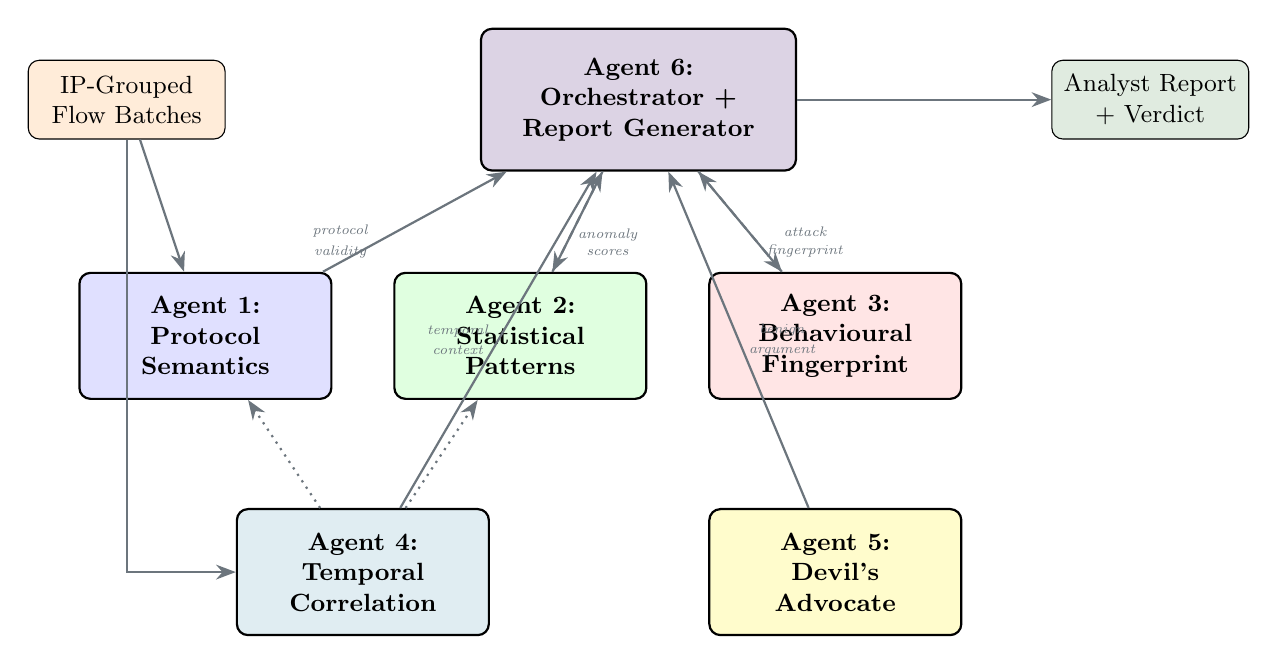
\begin{tikzpicture}[
  agent/.style={draw, rounded corners=4pt, minimum width=3.2cm,
    minimum height=1.6cm, align=center, font=\small\bfseries,
    line width=0.8pt},
  orch/.style={agent, fill=UQpurple!20, minimum width=4cm,
    minimum height=1.8cm},
  flow/.style={-{Stealth[length=2.5mm]}, thick, color=codegray},
  label/.style={font=\tiny\itshape, color=codegray},
]
  % Orchestrator at top
  \node[orch] (orch) at (6.5,6)
    {Agent 6:\\Orchestrator +\\Report Generator};

  % Input
  \node[draw, rounded corners, fill=orange!15, minimum width=2.5cm,
    minimum height=1cm, align=center, font=\small] (input) at (0,6)
    {IP-Grouped\\Flow Batches};

  % Row 1: Analysis agents
  \node[agent, fill=blue!12] (proto) at (1,3)
    {Agent 1:\\Protocol\\Semantics};
  \node[agent, fill=green!12] (stats) at (5,3)
    {Agent 2:\\Statistical\\Patterns};
  \node[agent, fill=red!10] (behav) at (9,3)
    {Agent 3:\\Behavioural\\Fingerprint};

  % Row 2: Context agents
  \node[agent, fill=accent!15] (temporal) at (3,0)
    {Agent 4:\\Temporal\\Correlation};
  \node[agent, fill=yellow!20] (devil) at (9,0)
    {Agent 5:\\Devil's\\Advocate};

  % Output
  \node[draw, rounded corners, fill=codegreen!15, minimum width=2.5cm,
    minimum height=1cm, align=center, font=\small] (output) at (13,6)
    {Analyst Report\\+ Verdict};

  % Arrows from input
  \draw[flow] (input) -- (proto);
  \draw[flow] (input) |- (temporal);

  % Agents to orchestrator
  \draw[flow] (proto) -- node[label, left, pos=0.3] {\shortstack{protocol\\validity}} (orch);
  \draw[flow] (stats) -- node[label, right, pos=0.3] {\shortstack{anomaly\\scores}} (orch);
  \draw[flow] (behav) -- node[label, right, pos=0.3] {\shortstack{attack\\fingerprint}} (orch);
  \draw[flow] (temporal) -- node[label, left, pos=0.5] {\shortstack{temporal\\context}} (orch);
  \draw[flow] (devil) -- node[label, right, pos=0.5] {\shortstack{benign\\argument}} (orch);

  % Orchestrator distributes to analysis agents
  \draw[flow, dashed] (orch) -- (stats);
  \draw[flow, dashed] (orch) -- (behav);

  % Temporal feeds context to analysis agents
  \draw[flow, dotted] (temporal) -- (proto);
  \draw[flow, dotted] (temporal) -- (stats);

  % Output
  \draw[flow] (orch) -- (output);
\end{tikzpicture}
\caption{AMATAS six-agent architecture. Solid arrows show data flow;
  dashed arrows show orchestrator distribution; dotted arrows show
  temporal context injection. All agents use pure LLM reasoning---no
  external APIs.}
\label{fig:amatas}
\end{figure}


\section{Agent Specifications}

\subsection{Agent 1: Protocol Semantics Agent}

\begin{table}[H]
\centering
\begin{tabular}{@{}lp{10cm}@{}}
\toprule
\textbf{Asks}     & ``Is this traffic protocol-valid? Does the flow conform to
                     expected protocol behaviour for the indicated ports and
                     flags?'' \\
\textbf{Receives}  & Individual flow records with all 53 features \\
\textbf{Outputs}   & Protocol compliance score (0--1), list of violations,
                     expected vs.\ observed behaviour \\
\textbf{Addresses} & \emph{Phase 1 Tier 3 failures:} Infiltration flows that
                     mimicked DNS (port 53, valid query structure) were missed
                     because the baseline agent accepted protocol-valid flows
                     as benign. This agent flags \emph{contextually inappropriate}
                     protocol usage (e.g., DNS AAAA queries at machine speed). \\
\bottomrule
\end{tabular}
\end{table}

\subsection{Agent 2: Statistical Pattern Agent}

\begin{table}[H]
\centering
\begin{tabular}{@{}lp{10cm}@{}}
\toprule
\textbf{Asks}     & ``Are the numbers anomalous? Do byte counts, packet ratios,
                     duration, and flag distributions fall within normal ranges?'' \\
\textbf{Receives}  & Flow features + temporal baseline statistics from Agent 4 \\
\textbf{Outputs}   & Anomaly score per feature, z-scores against temporal baseline,
                     top-3 anomalous features with explanation \\
\textbf{Addresses} & \emph{Phase 1 Tiers 1--2:} The baseline agent detected
                     volume-based attacks (DDoS, DoS) through implicit statistical
                     reasoning. This agent makes that reasoning \emph{explicit}
                     and \emph{calibrated}, with quantified deviation from
                     established baselines rather than ad-hoc feature inspection. \\
\bottomrule
\end{tabular}
\end{table}

\subsection{Agent 3: Behavioural Fingerprint Agent}

\begin{table}[H]
\centering
\begin{tabular}{@{}lp{10cm}@{}}
\toprule
\textbf{Asks}     & ``What attack pattern does this match? Given the flow
                     characteristics, which known attack type (if any) best
                     explains the observed behaviour?'' \\
\textbf{Receives}  & Flow features + anomaly scores from Agent 2 \\
\textbf{Outputs}   & Top-3 candidate attack types with confidence, MITRE ATT\&CK
                     technique mapping, differential diagnosis (why attack X
                     rather than attack Y) \\
\textbf{Addresses} & \emph{Phase 1 misclassifications:} The baseline agent
                     frequently identified the correct \emph{indicators} but
                     mapped them to wrong attack types (e.g., SSH brute force
                     labelled as FTP probing). This agent specialises in
                     attack-signature matching and provides structured
                     differential diagnosis. \\
\bottomrule
\end{tabular}
\end{table}

\subsection{Agent 4: Temporal Correlation Agent}

\begin{table}[H]
\centering
\begin{tabular}{@{}lp{10cm}@{}}
\toprule
\textbf{Asks}     & ``What happened before and after this flow? Does this IP's
                     activity over the time window show suspicious patterns?'' \\
\textbf{Receives}  & IP-grouped flow batches (all flows from same source IP
                     within a time window, ordered chronologically) \\
\textbf{Outputs}   & Temporal baseline per IP (normal behaviour profile),
                     burst detection alerts, behavioural change flags,
                     retroactive reclassification triggers \\
\textbf{Addresses} & \emph{Phase 1 Tier 3 and Phase 2 Iter 1:} Infiltration
                     attacks (30 DNS queries in 3.2\,s) and XSS brute force
                     (repeated DHCP-like flows) were invisible to single-flow
                     analysis. Iter 1's temporal memory improved benign accuracy
                     but lacked selectivity. This agent maintains per-IP temporal
                     state as a \emph{first-class analytical function}, not just
                     a tool. \\
\bottomrule
\end{tabular}
\end{table}

\subsection{Agent 5: Devil's Advocate Agent}

\begin{table}[H]
\centering
\begin{tabular}{@{}lp{10cm}@{}}
\toprule
\textbf{Asks}     & ``What is the strongest benign explanation for this traffic?
                     Assuming this flow is legitimate, what normal behaviour
                     would produce these characteristics?'' \\
\textbf{Receives}  & Flow features + assessments from Agents 1--3 \\
\textbf{Outputs}   & Benign hypothesis with confidence, specific benign scenario
                     (e.g., ``automated backup to cloud storage''), evidence
                     supporting and contradicting the benign interpretation \\
\textbf{Addresses} & \emph{Phase 1 Tier 4 and Phase 2 Iter 2:} The baseline's
                     13.3\% benign accuracy stemmed from a suspicious-by-default
                     bias---the agent had no mechanism to argue \emph{for} benign.
                     Iter 2's benign calibration attempted to encode this in the
                     prompt but was too rigid. The Devil's Advocate provides
                     a dedicated adversarial voice that forces the orchestrator
                     to weigh benign explanations against attack hypotheses. \\
\bottomrule
\end{tabular}
\end{table}

\subsection{Agent 6: Orchestrator + Analyst Report Generator}

\begin{table}[H]
\centering
\begin{tabular}{@{}lp{10cm}@{}}
\toprule
\textbf{Asks}     & ``Given all agent assessments, what is the final verdict?
                     How should this be communicated to a SOC analyst?'' \\
\textbf{Receives}  & Structured outputs from all five specialist agents \\
\textbf{Outputs}   & Final verdict (BENIGN/SUSPICIOUS/MALICIOUS), confidence
                     (0--1), attack type classification, MITRE mapping,
                     natural-language analyst report with evidence chain,
                     retroactive reclassification decisions \\
\textbf{Addresses} & \emph{Phase 2 Iter 3 override failure:} The confidence
                     override was a single global threshold applied post-hoc.
                     The orchestrator instead mediates between agents with
                     competing assessments (e.g., Agent 2 says anomalous, Agent 5
                     says benign DNS). The verdict emerges from structured
                     deliberation, not thresholding. \\
\bottomrule
\end{tabular}
\end{table}


\section{Design Principles}

\begin{enumerate}
  \item \textbf{Pure LLM reasoning.} No external API calls, no ML pre-filter.
        All classification is performed by LLM agents reasoning over flow
        features and each other's outputs. This eliminates the tool-dependency
        problem demonstrated in Phase 1, testing whether LLMs' intrinsic
        pre-trained knowledge suffices for detection~\cite{houssel2024towards}.

  \item \textbf{Adversarial deliberation.} The Devil's Advocate (Agent 5)
        ensures that every suspicious verdict must overcome a structured benign
        counter-argument. This replaces the prompt-level calibration of Phase 2
        with an agent-level dialectic, following Tran et al.'s finding that
        systems combining competition and cooperation are most
        effective~\cite{tran2025collaboration}.

  \item \textbf{Temporal-first design.} Flows are grouped by source IP and
        presented chronologically to Agent 4 \emph{before} individual analysis.
        This inverts the Phase 1 approach where temporal context was an
        afterthought, and addresses the SagaLLM finding that LLMs ``lack native
        mechanisms to maintain state''~\cite{sagallm2025} by architecturally
        separating temporal reasoning.

  \item \textbf{Structured disagreement.} When agents disagree (e.g., Agent 2
        flags statistical anomaly but Agent 5 provides a compelling benign
        explanation), the orchestrator must explicitly resolve the disagreement
        with reasoning, rather than applying a threshold. Quan et
        al.~\cite{quan2024collaboration} found that team structure critically
        impacts multi-agent performance.

  \item \textbf{Explainability by construction.} Every verdict includes a
        complete evidence chain: which agents contributed, what they found,
        where they disagreed, and how the orchestrator resolved conflicts.
        This produces analyst-ready reports following the explainer paradigm
        established by eX-NIDS~\cite{houssel2025exnids} and
        HuntGPT~\cite{ali2023huntgpt}.
\end{enumerate}


\section{Failure Mode Coverage}

\begin{table}[H]
\centering
\caption{How each AMATAS agent addresses Phase 1--2 failure modes}
\label{tab:failure-coverage}
\small
\begin{tabular}{@{}p{4cm}cp{6cm}@{}}
\toprule
\textbf{Failure Mode} & \textbf{Agent} & \textbf{Resolution} \\
\midrule
0\% external tool returns & All & No external tools used; pure LLM reasoning \\
13.3\% benign accuracy & 5 & Devil's Advocate argues for benign interpretation \\
Infiltration missed (DNS burst) & 4 & Temporal agent detects 30-query burst \\
XSS disguised as DHCP & 1, 4 & Protocol agent flags contextual violations;
  temporal agent detects repetition rate \\
Attack normalisation (Iter 1) & 5, 6 & Devil's Advocate separated from temporal
  context; orchestrator mediates \\
Confidence override failure (Iter 3) & 6 & Structured deliberation replaces
  global threshold \\
97.7\% tool call errors (Iter 3) & All & No tool calls; agent-to-agent
  communication only \\
\$0.069--\$0.126/flow cost & 4 & IP-grouped batches amortise context across
  flows; temporal agent processes batches \\
\bottomrule
\end{tabular}
\end{table}


\section{Limitations}
\label{sec:limitations}

\subsection{Internal Validity}

\begin{itemize}
  \item \textbf{Small sample size:} 58 flows provide limited statistical power.
        Per-attack metrics (3 flows per type) cannot establish significance.
        Wilson score confidence intervals for 3/3 detection (100\%) span
        approximately [44\%, 100\%] at 95\% confidence.

  \item \textbf{Same test batch:} Using the same 58 flows across iterations
        risks overfitting to specific flow characteristics. Different flow
        selections might yield different relative rankings.

  \item \textbf{Prompt sensitivity:} The benign calibration prompt was designed
        based on observed failure modes. Different prompt formulations might
        produce different results.
\end{itemize}

\subsection{External Validity}

\begin{itemize}
  \item \textbf{Dataset representativeness:} CICIDS2018 is lab-generated with
        scripted attacks. Real-world traffic exhibits more noise, diversity,
        and adversarial evasion.

  \item \textbf{IP artefacts:} The 0\% external tool return rate is specific
        to this dataset. Contemporary datasets with real IPs would likely
        show non-zero tool utility.

  \item \textbf{Single LLM:} Results are specific to Claude Sonnet. Other
        models (GPT-4, Gemini, open-source) may exhibit different biases
        and performance profiles.
\end{itemize}

\subsection{Scalability}

At \$0.069--\$0.136/flow and 91--230\,s/flow, the approach does not scale
to production traffic volumes. The multi-agent architecture with hierarchical
triage is designed to address this, but has not yet been evaluated.


% =============================================================================
\chapter{Conclusion}
\label{ch:conclusion}
% =============================================================================

\section{Answers to Research Questions}

\paragraph{RQ1: Can NetFlow augmentation via MCP improve the detection performance
and explainability of LLM-based NIDS?}
No---not on historical datasets with anonymised IPs. The MCP architecture functioned
correctly (the agent discovered tools, constructed queries, and processed responses),
but external threat intelligence returned zero meaningful data across 142 queries
in Phase~1 and 97.7\% errors in Phase~2. The LLM's 83.3\% baseline F1 was driven
entirely by its intrinsic pre-trained knowledge of network security, not by tool
augmentation. MCP tool integration adds value only when the target IPs are
contemporary and present in threat databases---a condition that no historical
benchmark dataset satisfies. This finding reframes the MCP contribution: the
protocol is valuable as an \emph{inter-agent communication layer} (as demonstrated
in Phase~3), not as an external intelligence source for lab data.

\paragraph{RQ2: Can a multi-agent architecture of specialised LLM reasoning agents
match or exceed human analyst performance on network intrusion detection?}
Partially. Phase~3b demonstrated that AMATAS achieves 95.9\% F1 with 100\% recall
and 92.1\% precision on 150 flows---performance that approaches production-grade
NIDS requirements. The six-agent architecture resolved the single-agent ceiling
identified in Phase~2: where no single-agent configuration could simultaneously
optimise precision, recall, and benign accuracy, the multi-agent system achieved
100\% benign accuracy and 100\% recall (though not in the same batch). However,
Phase~3c exposed a persistent weakness at realistic benign-heavy distributions
(54.0\% accuracy, 41 false positives on 88 benign flows), indicating that the
Devil's Advocate agent requires further calibration before the system can operate
in production environments where 85\%+ of traffic is benign.


\section{Summary}

This thesis investigated whether Large Language Models can perform network
intrusion detection through structured reasoning over NetFlow features. Three
phases of experimentation---single-agent with MCP tools, iterative single-agent
improvements, and a six-agent multi-agent architecture---produced three principal
findings. First, LLMs possess substantial intrinsic capability for flow-level
threat detection: the baseline agent achieved 83.3\% F1 using only pre-trained
knowledge, with zero contribution from external tool augmentation. Second,
single-agent architectures hit a fundamental ceiling where precision, recall, and
benign accuracy cannot be simultaneously optimised through prompt engineering
alone---Iteration~3's confidence override collapsed F1 to 45.2\% by suppressing
true positives. Third, multi-agent decomposition breaks through this ceiling:
AMATAS achieved 95.9\% F1 at scale (Phase~3b) by assigning specialised analytical
roles to six agents whose structured disagreement replaces brittle thresholding.

These findings mean that LLM-based NIDS is viable as an analytical capability,
not as a replacement for high-throughput statistical classifiers. The value
proposition is explainability: every AMATAS verdict includes a complete evidence
chain---which agents contributed, what they found, where they disagreed, and how
the orchestrator resolved conflicts. This produces analyst-ready reports that no
ML classifier can match. The architecture also demonstrates that pure LLM reasoning,
without fine-tuning or external intelligence, can detect 6 of 14 attack types with
100\% accuracy across 308 flows.

The path forward requires three advances. The Devil's Advocate must be tuned to
reduce its 33.3\% incorrect flip rate, particularly on DoS/DDoS flows where it
currently suppresses true positives. Cross-dataset validation on
UNSW-NB15~\cite{moustafa2015unswnb15} is essential to demonstrate that AMATAS
generalises beyond CICIDS2018's known limitations~\cite{engelen2021cicids}. And
hierarchical triage---routing high-confidence flows through a lightweight
pre-filter and reserving the six-agent pipeline for ambiguous cases---is the
scalability path that makes \$0.070/flow economically viable at production
volumes.


\section{Future Work}

\begin{enumerate}
  \item \textbf{Devil's Advocate calibration.} The current 66.7\% flip accuracy
        leaves room for improvement. Potential approaches include providing the
        Devil's Advocate with statistical baselines from Agent~2 (so it argues
        benign only when features are within normal ranges), or introducing a
        confidence threshold below which flips are not permitted. The goal is to
        maintain the false-positive elimination observed in Phase~3a while
        reducing the false-negative introduction on DoS/DDoS flows.

  \item \textbf{Cross-dataset validation on UNSW-NB15.} All evaluation in this
        thesis uses CICIDS2018, which has documented flow construction
        errors~\cite{engelen2021cicids, liu2022errors}, class
        imbalance~\cite{panigrahi2018cicids}, and transferability
        concerns~\cite{transferability2022}. Evaluating AMATAS on
        UNSW-NB15~\cite{moustafa2015unswnb15}---which offers more realistic
        normal traffic and modern attack types---would establish whether the
        architecture generalises across datasets or is inadvertently tuned to
        CICIDS2018's characteristics.

  \item \textbf{Scalability via hierarchical triage.} The current \$0.070/flow
        cost assumes every flow passes through all six agents. A production
        deployment would route statistically obvious flows (Tiers~1--2) through
        a lightweight pre-filter, engaging the full AMATAS pipeline only for
        ambiguous flows. Phase~1's finding that 75\% of attacks have strong
        statistical signatures suggests that 90\%+ of flows could be classified
        without LLM involvement, reducing effective per-flow cost by an order of
        magnitude.
\end{enumerate}


% =============================================================================
% APPENDICES
% =============================================================================
\appendix

\chapter{Per-Flow Reasoning Examples}
\label{app:reasoning}

Selected per-flow reasoning from the Phase 1 evaluation, illustrating the
agent's decision-making process.

\subsection{True Positive: FTP Brute Force (Flow 3)}

\begin{quote}
\small\itshape
``Three consecutive FTP flows, same target, incrementing source ports
(39924$\rightarrow$39934$\rightarrow$40030). IP history confirms repeated
brute-force pattern. Observation recorded: service enumeration behaviour.''
\end{quote}

\textbf{Analysis:} The agent correctly identified the brute-force signature
(incrementing ports, same target) and used the \texttt{get\_ip\_history} tool
to confirm the pattern. Confidence: 0.50 (SUSPICIOUS).

\subsection{False Negative: Infiltration via DNS (Flow 50)}

\begin{quote}
\small\itshape
``Single DNS AAAA query from internal IP. Agent correctly identified as
legitimate DNS. But this is part of a 30-flow burst from 2 IPs in 3.2
seconds---temporal context required.''
\end{quote}

\textbf{Analysis:} The agent's flow-level reasoning was correct---a single DNS
query \emph{is} benign in isolation. The attack signature exists only in the
temporal domain (30 queries in 3.2\,s), which the baseline agent cannot observe.

\subsection{False Positive: Benign DNS (Flow 7)}

\begin{quote}
\small\itshape
``Single DNS A record query. Private RFC1918 addressing. Normal packet sizes
(69/85 bytes). Agent flagged suspicious despite no anomalies---false positive
from over-cautious base behaviour.''
\end{quote}

\textbf{Analysis:} The agent's reasoning identified no anomalies but still
produced a SUSPICIOUS verdict. This illustrates the suspicious-by-default bias
that drives the 13.3\% benign accuracy.


\chapter{Full Phase 2 Per-Attack Detection Rates}
\label{app:perattack}

\begin{table}[H]
\centering
\caption{Complete per-attack detection rates across all iterations}
\label{tab:full-perattack}
\small
\begin{tabular}{@{}lcccc@{}}
\toprule
\textbf{Attack Type} & \textbf{Baseline} & \textbf{Iter 1} & \textbf{Iter 2} & \textbf{Iter 3} \\
\midrule
Bot                   & 100\% (3/3) & 100\% (3/3) &  67\% (2/3) &  33\% (1/3) \\
Brute Force (Web)     & 100\% (3/3) &  67\% (2/3) & 100\% (3/3) &  33\% (1/3) \\
Brute Force (XSS)     &  67\% (2/3) &  67\% (2/3) &  33\% (1/3) &  67\% (2/3) \\
DDoS-HOIC             & 100\% (4/4) &  50\% (2/4) &  75\% (3/4) &   0\% (0/4) \\
DDoS-LOIC-UDP         & 100\% (3/3) & 100\% (3/3) & 100\% (3/3) &  33\% (1/3) \\
DDoS-LOIC-HTTP        & 100\% (3/3) &  33\% (1/3) &  67\% (2/3) &   0\% (0/3) \\
DoS-GoldenEye         & 100\% (3/3) &  67\% (2/3) &  67\% (2/3) &  33\% (1/3) \\
DoS-Hulk              & 100\% (3/3) &  67\% (2/3) &  33\% (1/3) &  33\% (1/3) \\
DoS-SlowHTTPTest      & 100\% (3/3) & 100\% (3/3) & 100\% (3/3) &  33\% (1/3) \\
DoS-Slowloris         & 100\% (3/3) &  33\% (1/3) &  33\% (1/3) &   0\% (0/3) \\
FTP-BruteForce        & 100\% (3/3) & 100\% (3/3) & 100\% (3/3) &  67\% (2/3) \\
Infiltration          &  33\% (1/3) &  67\% (2/3) & 100\% (3/3) &   0\% (0/3) \\
SQL Injection         & 100\% (3/3) &  33\% (1/3) & 100\% (3/3) &  67\% (2/3) \\
SSH-Bruteforce        & 100\% (3/3) &  67\% (2/3) & 100\% (3/3) &  67\% (2/3) \\
\midrule
Benign                &  13\% (2/15) &  67\% (10/15) &  40\% (6/15) &  67\% (10/15) \\
\bottomrule
\end{tabular}
\end{table}


% =============================================================================
% BIBLIOGRAPHY
% =============================================================================
\printbibliography[heading=bibintoc, title={References}]

\end{document}
